% Options for packages loaded elsewhere
\PassOptionsToPackage{unicode}{hyperref}
\PassOptionsToPackage{hyphens}{url}
\PassOptionsToPackage{dvipsnames,svgnames,x11names}{xcolor}
\documentclass[
  10.5pt,
  UTF8]{ctexart}
\usepackage{xcolor}
\usepackage[top=20mm,bottom=20mm,left=20mm,right=20mm]{geometry}
\usepackage{amsmath,amssymb}
\setcounter{secnumdepth}{-\maxdimen} % remove section numbering
\usepackage{iftex}
\ifPDFTeX
  \usepackage[T1]{fontenc}
  \usepackage[utf8]{inputenc}
  \usepackage{textcomp} % provide euro and other symbols
\else % if luatex or xetex
  \usepackage{unicode-math} % this also loads fontspec
  \defaultfontfeatures{Scale=MatchLowercase}
  \defaultfontfeatures[\rmfamily]{Ligatures=TeX,Scale=1}
\fi
\usepackage{lmodern}
\ifPDFTeX\else
  % xetex/luatex font selection
\fi
% Use upquote if available, for straight quotes in verbatim environments
\IfFileExists{upquote.sty}{\usepackage{upquote}}{}
\IfFileExists{microtype.sty}{% use microtype if available
  \usepackage[]{microtype}
  \UseMicrotypeSet[protrusion]{basicmath} % disable protrusion for tt fonts
}{}
\makeatletter
\@ifundefined{KOMAClassName}{% if non-KOMA class
  \IfFileExists{parskip.sty}{%
    \usepackage{parskip}
  }{% else
    \setlength{\parindent}{0pt}
    \setlength{\parskip}{6pt plus 2pt minus 1pt}}
}{% if KOMA class
  \KOMAoptions{parskip=half}}
\makeatother
\usepackage{longtable,booktabs,array}
\newcounter{none} % for unnumbered tables
\usepackage{calc} % for calculating minipage widths
% Correct order of tables after \paragraph or \subparagraph
\usepackage{etoolbox}
\makeatletter
\patchcmd\longtable{\par}{\if@noskipsec\mbox{}\fi\par}{}{}
\makeatother
% Allow footnotes in longtable head/foot
\IfFileExists{footnotehyper.sty}{\usepackage{footnotehyper}}{\usepackage{footnote}}
\makesavenoteenv{longtable}
\usepackage{graphicx}
\makeatletter
\newsavebox\pandoc@box
\newcommand*\pandocbounded[1]{% scales image to fit in text height/width
  \sbox\pandoc@box{#1}%
  \Gscale@div\@tempa{\textheight}{\dimexpr\ht\pandoc@box+\dp\pandoc@box\relax}%
  \Gscale@div\@tempb{\linewidth}{\wd\pandoc@box}%
  \ifdim\@tempb\p@<\@tempa\p@\let\@tempa\@tempb\fi% select the smaller of both
  \ifdim\@tempa\p@<\p@\scalebox{\@tempa}{\usebox\pandoc@box}%
  \else\usebox{\pandoc@box}%
  \fi%
}
% Set default figure placement to htbp
\def\fps@figure{htbp}
\makeatother
\ifLuaTeX
\usepackage[bidi=basic,shorthands=off,provide=*]{babel}
\else
\usepackage[bidi=default,shorthands=off,provide=*]{babel}
\fi
\ifLuaTeX
  \usepackage{selnolig} % disable illegal ligatures
\fi
\setlength{\emergencystretch}{3em} % prevent overfull lines
\providecommand{\tightlist}{%
  \setlength{\itemsep}{0pt}\setlength{\parskip}{0pt}}
\usepackage{bookmark}
\IfFileExists{xurl.sty}{\usepackage{xurl}}{} % add URL line breaks if available
\urlstyle{same}
% fallback for those not using the hyperref driver hyperxmp:
\makeatletter
\@ifundefined{xmpquote}{\newcommand{\xmpquote}[1]{#1}}{}
\makeatother
\hypersetup{
  pdftitle={DeepBlock：拓扑共设计的量子局部搜索},
  pdfauthor={参赛团队（姓名、单位待补）},
  pdflang={zh-CN},
  colorlinks=true,
  linkcolor={blue},
  filecolor={Maroon},
  citecolor={Blue},
  urlcolor={blue},
  pdfcreator={LaTeX via pandoc}}

\title{DeepBlock：拓扑共设计的量子局部搜索}
\usepackage{etoolbox}
\makeatletter
\providecommand{\subtitle}[1]{% add subtitle to \maketitle
  \apptocmd{\@title}{\par {\large #1 \par}}{}{}
}
\makeatother
\subtitle{Baihua真机上的CVRP闭环证据}
\author{参赛团队（姓名、单位待补）}
\date{量子+优化赛道半决赛论文 · 2026年8月}

\begin{document}
\maketitle

\section{摘要}\label{ux6458ux8981}

在当前量子硬件上做组合优化，最容易得到的是``线路运行成功''，最难回答的是``量子样本究竟贡献了什么''。本项目以容量约束车辆路径问题（CVRP）为对象，提出DeepBlock拓扑共设计混合精化框架：经典端先构造容量可行路线，从相邻车辆边界提取16位客户，并组成三个最多8变量、相邻重叠3客户的局部块；量子端将局部重分配编码为稀疏QUBO，使每条保留的二次项直接对应Baihua处理器上的物理耦合；测量结果返回后，经典端只负责容量修复、真实路线距离计算与严格改善接受。

论文没有用最终路线结果反推量子贡献，而是给量子核设置独立门槛：对每个8比特QUBO精确枚举256个状态，将能量最低的26个状态预定义为高质量区。Baihua真机在该区域的平均概率质量为27.76\%，均匀随机为10.16\%，理想QAOA为39.18\%。因此，真机相对同一QUBO上的均匀随机实现2.73倍低能富集，增加17.60个百分点；6/6个独立种子方向一致，精确符号翻转检验\(p=0.03125\)。换句话说，真实硬件保留了理想QAOA``超出随机部分''的60.6\%，并非输出近似均匀的bitstring。

正式实验执行36个Baihua任务，每任务4,096 shots，总计147,456 shots；全部任务0 SWAP，平均线路深度27.7，平均双量子位门层数13.3。量子候选进入完整CVRP闭环后，在6/6个有局部余量的40客户、4车辆实例上产生严格改善，平均恢复71.4\%的局部精确余量。项目同时保存任务ID、校准快照、逻辑与物理QASM、物理映射、原始counts和状态转移，并完成144/144条离线重放。本文的核心结论不是量子加速，而是一个更适合现阶段硬件、也更容易由评委复核的事实：\textbf{Baihua真机在拓扑共设计QUBO上形成了显著的低能采样偏置，这一偏置已经被接入真实约束、真实目标和单调接受组成的优化闭环。}

\textbf{关键词：} CVRP；QAOA；QUBO；量子-经典混合优化；超导量子计算；候选质量；拓扑共设计

\begin{figure}
\centering
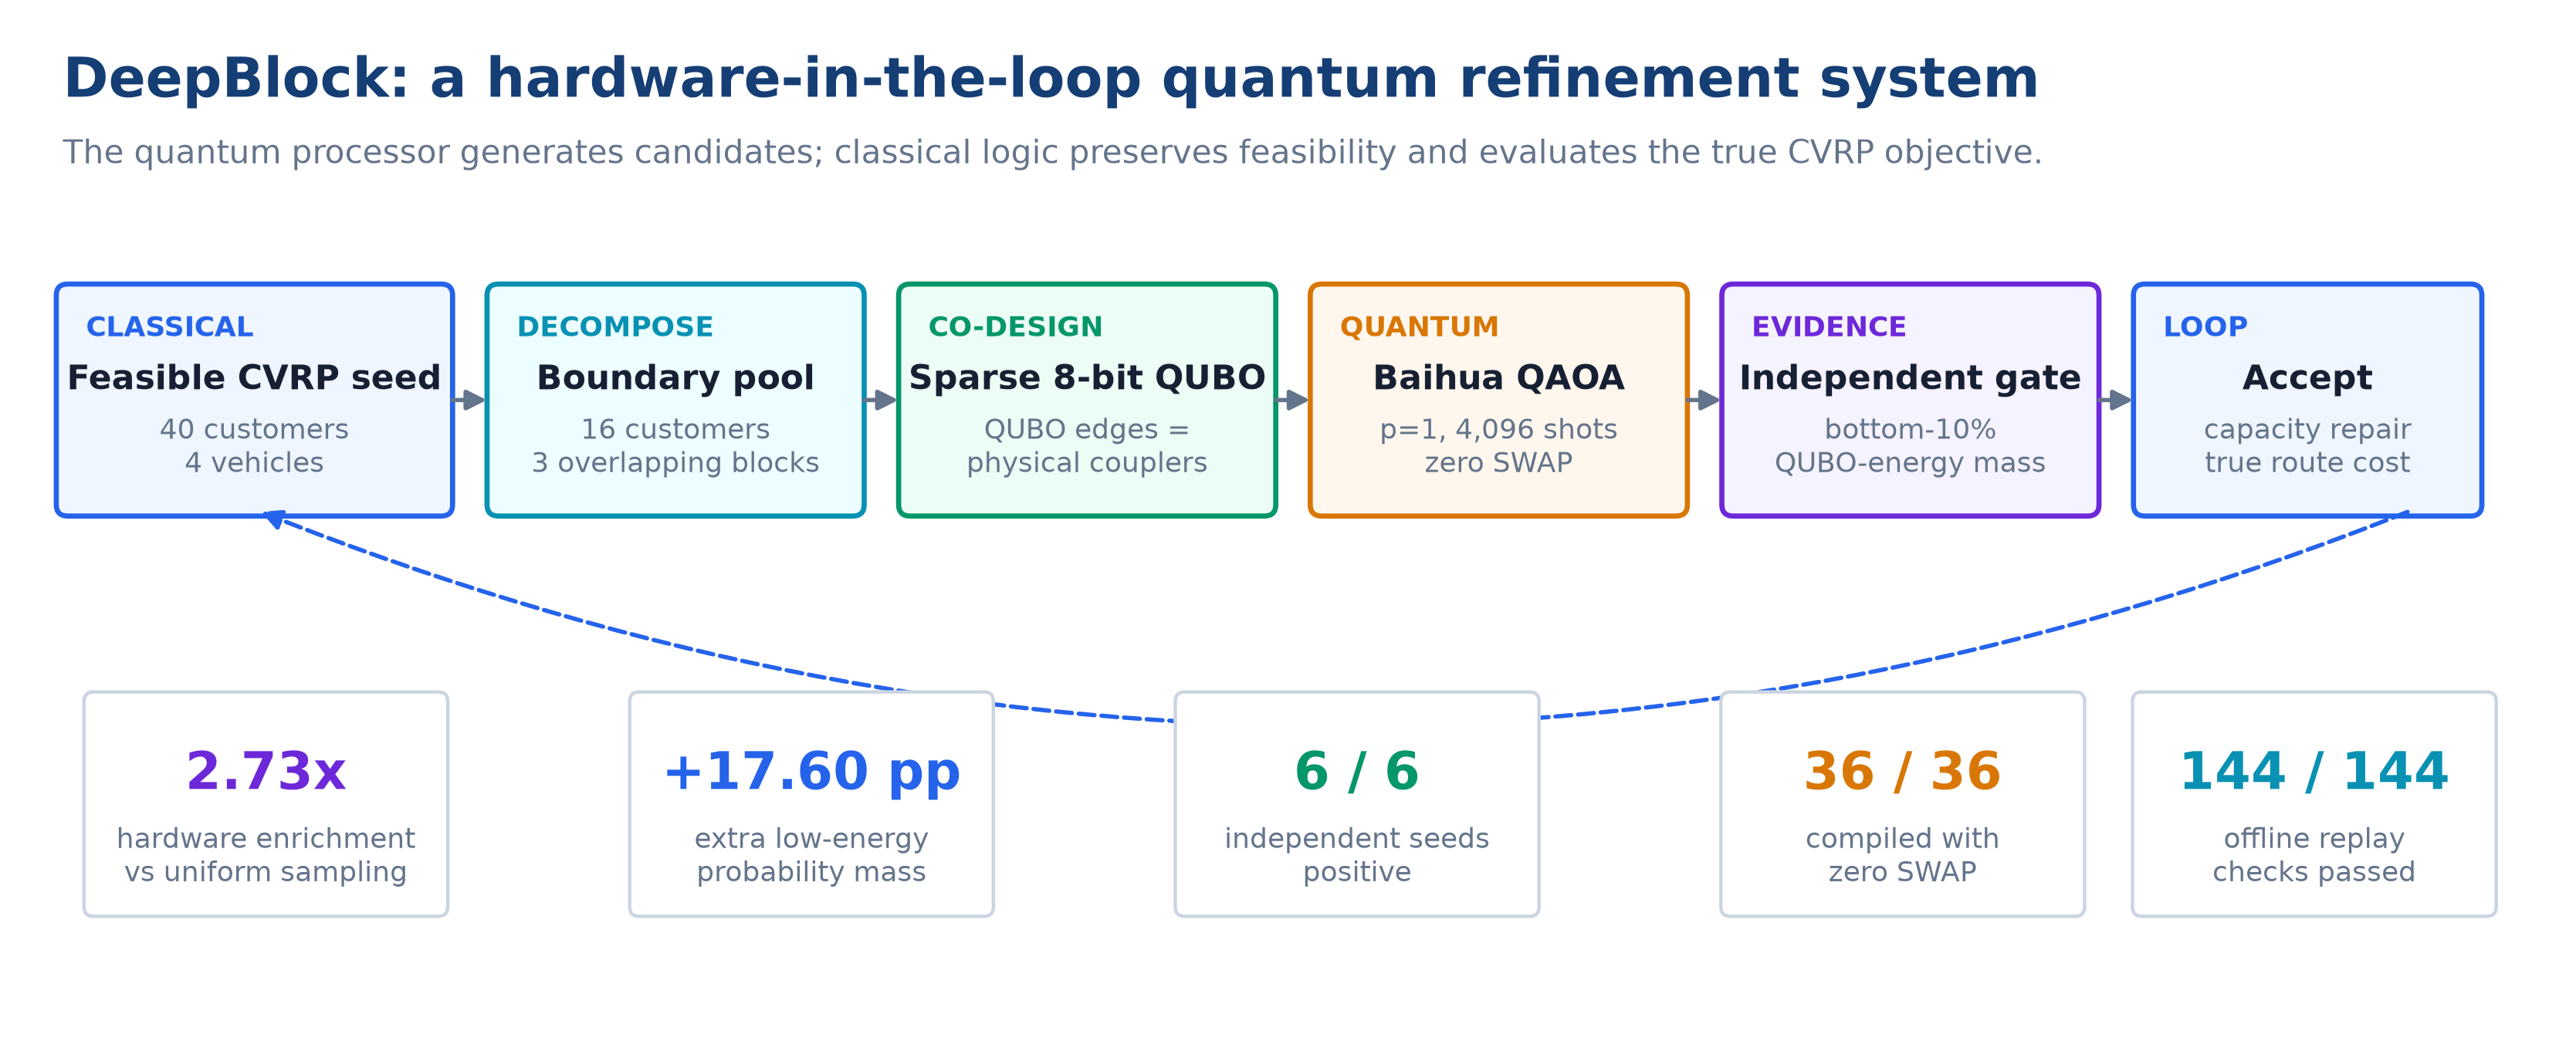
\includegraphics[width=1\linewidth,height=\textheight,keepaspectratio]{figures/fig01_graphical_abstract.png}
\caption{DeepBlock系统总览与核心结果。量子处理器只承担候选生成，经典端承担约束与真实目标；这使量子贡献能够被单独检验。}
\end{figure}

\section{1. 评委真正需要判断的问题}\label{ux8bc4ux59d4ux771fux6b63ux9700ux8981ux5224ux65adux7684ux95eeux9898}

CVRP同时包含客户分配、访问顺序、车辆容量和子回路约束。直接位置编码通常需要随客户数二次增长的量子位，还会产生稠密罚项；即使成功映射到小型设备，路由SWAP和线路深度也足以淹没低能信号。把完整40客户问题直接交给量子机，在今天并不是有雄心，而是没有把硬件限制写进算法。

DeepBlock选择另一条路线：让量子机进入一个它确实能影响、也能被独立考核的局部搜索位置。我们的判断不是``量子机能否替代OR-Tools''，而是以下三个递进问题：

\begin{enumerate}
\def\labelenumi{\arabic{enumi}.}
\tightlist
\item
  \textbf{量子分布是否有信息？} 在同一QUBO上，真机是否比均匀随机更集中于预先规定的低能区域？
\item
  \textbf{信息是否进入优化闭环？} 这些样本经过可行性修复与真实路线评价后，是否真的改变CVRP状态？
\item
  \textbf{系统瓶颈在哪里？} 当前限制来自硬件噪声、代理目标错位，还是经典端只读取了太少的量子候选？
\end{enumerate}

这三个问题分别对应``量子性''\,``有效性''和``工程性''。只报告一个最优bitstring无法回答它们；只报告最终路线也无法区分量子采样、经典修复和接受规则的作用。因此，本文从一开始就把量子核证据与端到端证据拆开。

\begin{figure}
\centering
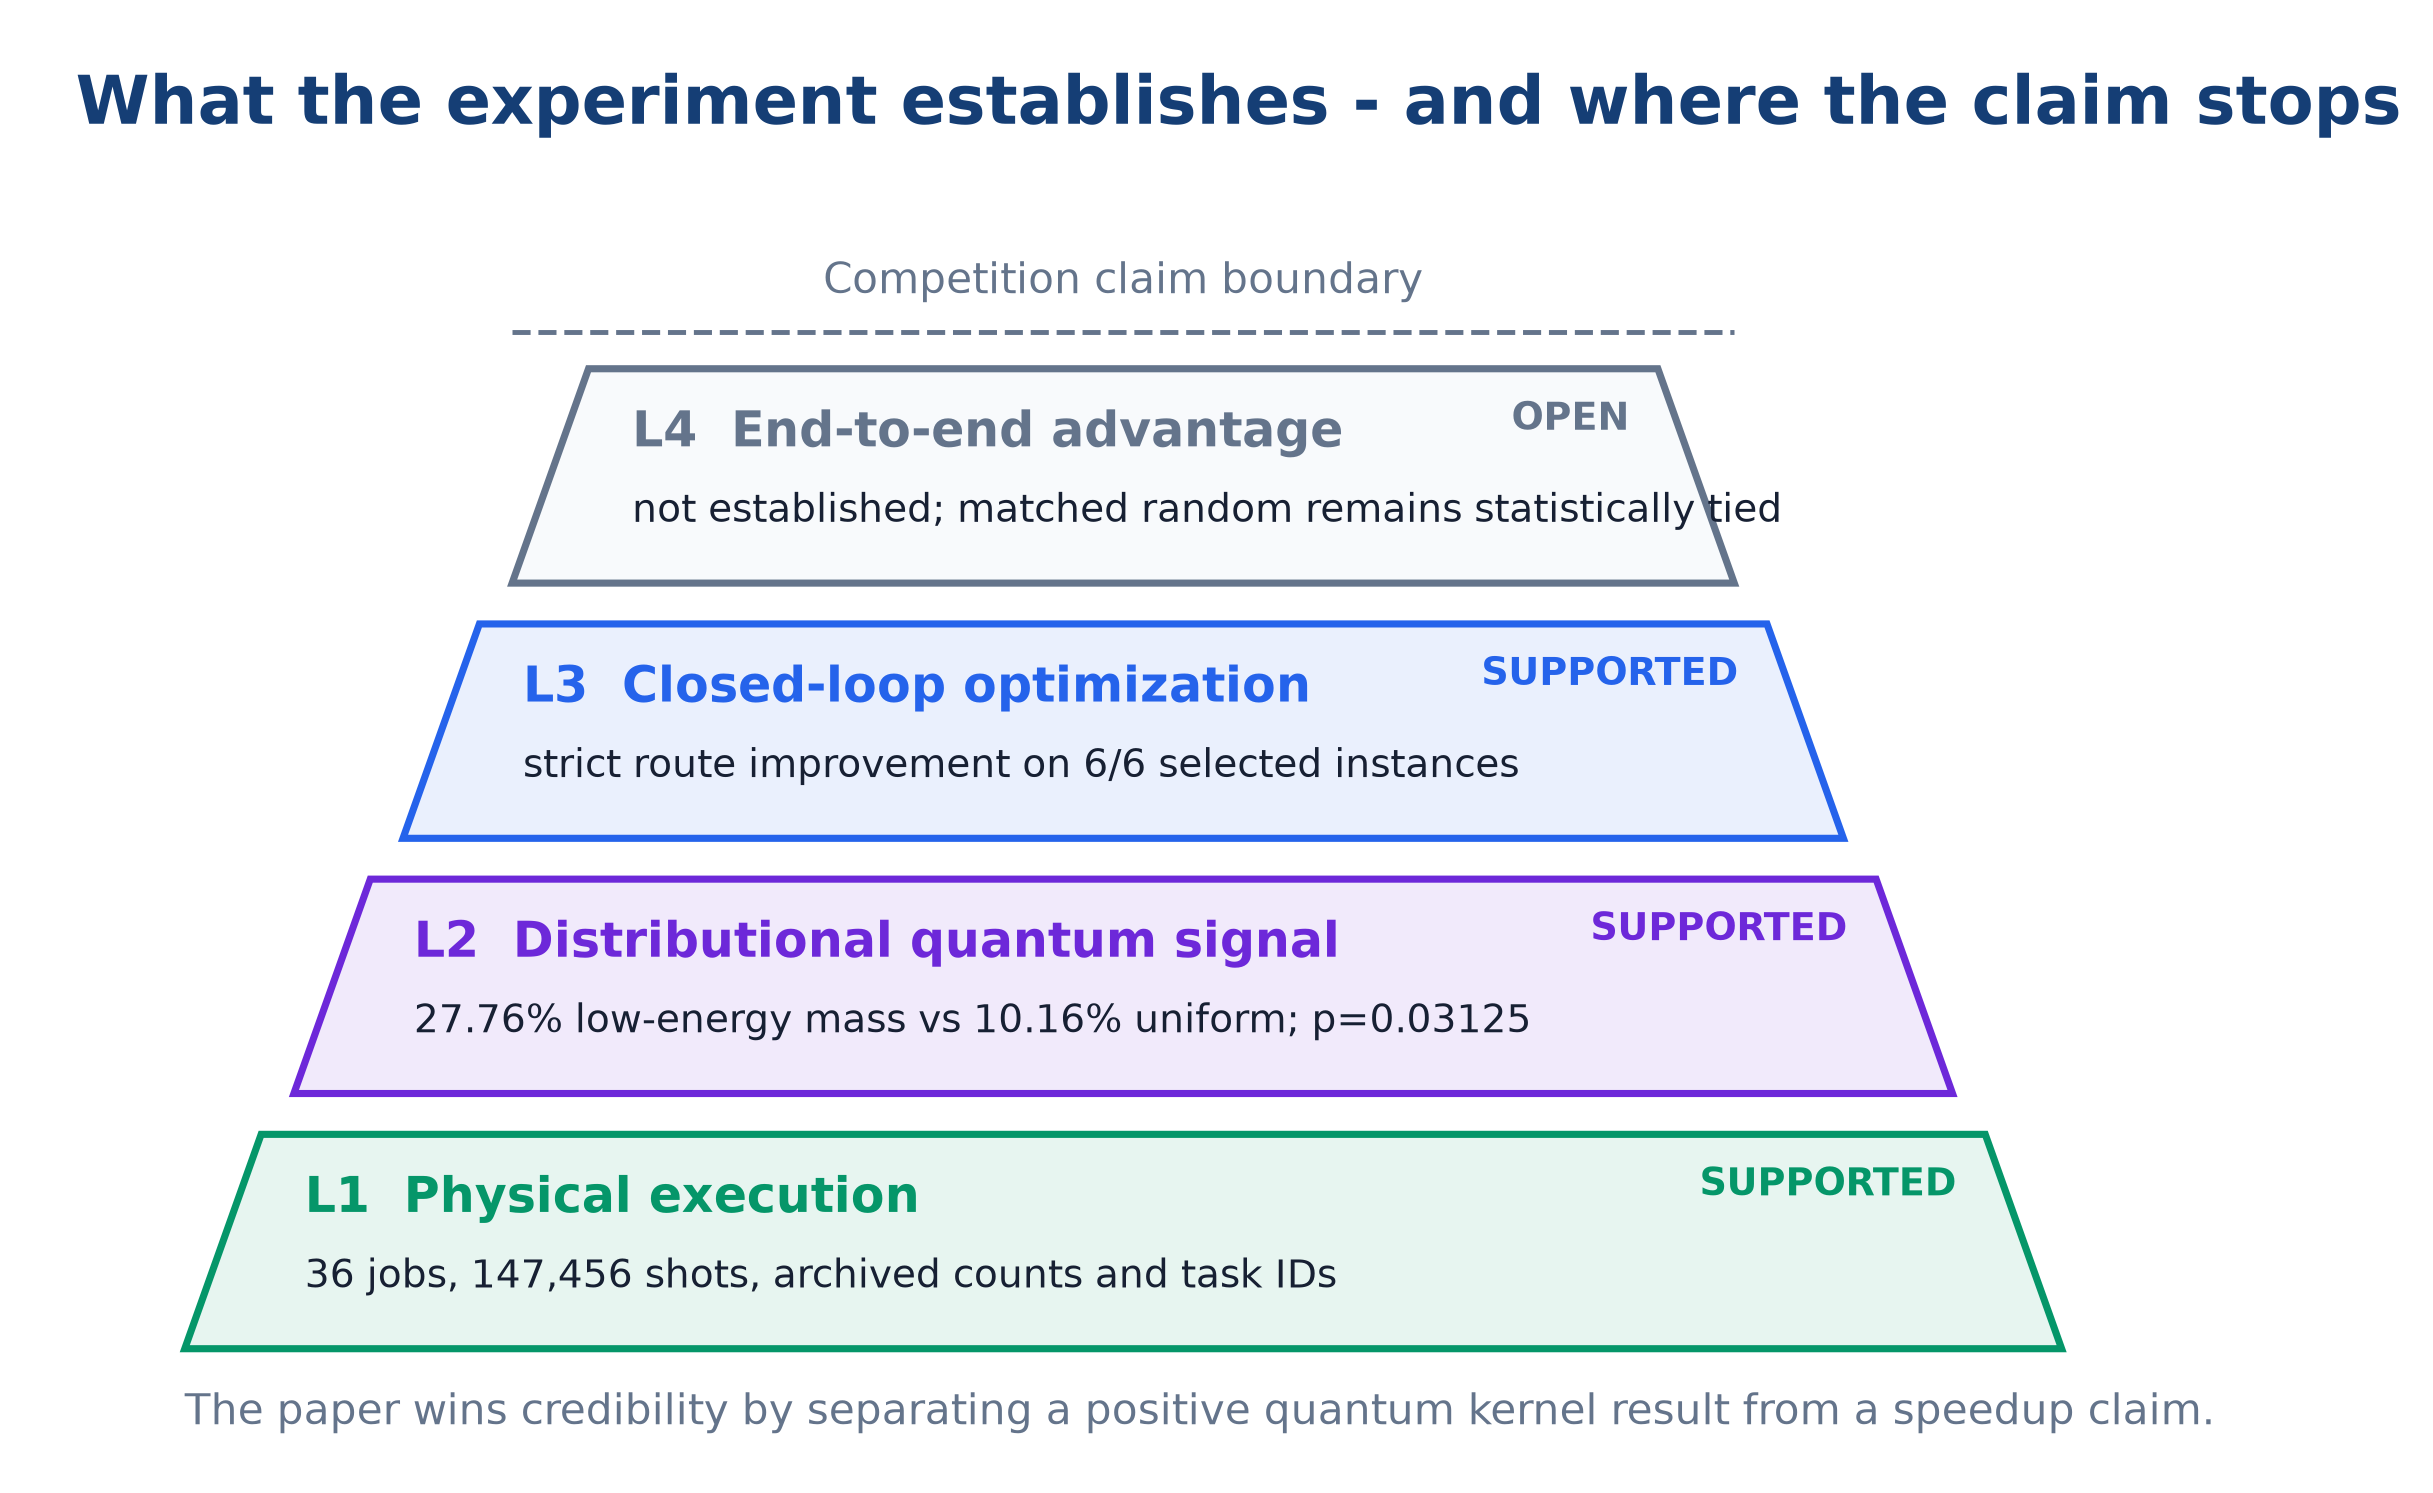
\includegraphics[width=0.84\linewidth,height=\textheight,keepaspectratio]{figures/fig02_evidence_ladder.png}
\caption{四层证据阶梯。项目已经完成物理执行、分布级量子信号和闭环优化三层证据；端到端量子优势不是本文主张。}
\end{figure}

\subsection{1.1 本项目的四项技术贡献}\label{ux672cux9879ux76eeux7684ux56dbux9879ux6280ux672fux8d21ux732e}

\textbf{贡献一：把量子贡献写成可否证的统计命题。} 每个量子子问题的``高质量区''只由QUBO能量排序决定，不读取真机counts，也不依赖路线是否接受。若Baihua没有形成低能偏置，27.76\%这一数值会退回10.16\%附近，结论自然失败。

\textbf{贡献二：从建模阶段消除路由开销。} 我们不是先构造稠密QUBO再让编译器补救，而是先选Baihua高保真物理链，再只保留链上直接耦合对应的二次项。正式任务使用物理量子位\([41,28,29,30,17,16,15,14]\)，36/36个真机线路不需要SWAP。

\textbf{贡献三：让真机counts逐块改变后续问题。} 三个重叠DeepBlock采用\(B_1\rightarrow B_2\rightarrow B_3\rightarrow B_3\rightarrow B_2\rightarrow B_1\)双向扫描。前一块接受的客户分配会改变后一块的QUBO，因此36次硬件调用不是一次静态演示，而是hardware-in-the-loop状态演化。

\textbf{贡献四：把失败信息变成工程结论。} \(p=2\)在个别种子恢复更多精确余量，却没有稳定改善；相反，把\(p=1\)的候选预算从\(k=8\)扩展到\(k=64\)，使种子2/3/4的真机平均路线改进从1.593增至3.475。现阶段最先该修的不是线路深度，而是量子代理与真实路线目标的对齐，以及如何使用长尾低频样本。

\section{2. 问题、边界与混合分工}\label{ux95eeux9898ux8fb9ux754cux4e0eux6df7ux5408ux5206ux5de5}

\subsection{2.1 CVRP与局部重分配}\label{cvrpux4e0eux5c40ux90e8ux91cdux5206ux914d}

设仓库为节点0，客户集合为\(V=\{1,\ldots,n\}\)，车辆集合为\(K=\{1,\ldots,m\}\)，客户需求为\(d_i\)，车辆容量为\(Q\)，节点间距离为\(c_{ij}\)。完整CVRP的路线目标为

\[
\min \sum_{k\in K}\sum_{i,j\in V\cup\{0\}} c_{ij}y_{ijk},
\]

其中\(y_{ijk}=1\)表示车辆\(k\)从节点\(i\)行驶到节点\(j\)。完整模型还需满足一次访问、流守恒、容量和子回路消除约束。

DeepBlock固定大部分当前解，只在一对相邻车辆\(a,b\)之间重新分配局部客户块\(B=\{v_1,\ldots,v_w\}\)，\(w\le 8\)。二进制变量\(x_i=0\)表示客户\(v_i\)属于车辆\(a\)，\(x_i=1\)表示属于车辆\(b\)。量子端优化的是稀疏代理能量

\[
E_Q(\mathbf{x})=c+\sum_{i=1}^{w}h_i x_i+\sum_{(i,j)\in\mathcal{E}_{\mathrm{phy}}}J_{ij}x_i x_j,
\]

其中\(\mathcal{E}_{\mathrm{phy}}\)不是任意完全图，而是选定物理链支持的逻辑边集合。线性项综合边界几何和负载变化，二次项表示客户共同移动的相互作用。代理能量用于塑造采样分布，最终接受仍以完整CVRP路线距离为准。

\subsection{2.2 为什么必须保留经典端}\label{ux4e3aux4ec0ux4e48ux5fc5ux987bux4fddux7559ux7ecfux5178ux7aef}

量子核输出的是局部二进制重分配，不直接承诺容量可行，也不直接包含完整访问顺序。若把容量修复和路径重建隐藏在``量子算法''内部，任何路线改善都无法归因。因此我们明确划分职责：

{\def\LTcaptype{none} % do not increment counter
\begin{longtable}[]{@{}lcc@{}}
\toprule\noalign{}
环节 & 量子端 & 经典端 \\
\midrule\noalign{}
\endhead
\bottomrule\noalign{}
\endlastfoot
低能局部分配候选生成 & 是 & 随机/模拟/精确对照 \\
容量约束检查与确定性修复 & 否 & 是 \\
路线重建与2-opt & 否 & 是 \\
完整距离目标计算 & 否 & 是 \\
严格改善接受与状态更新 & 否 & 是 \\
QUBO低能区域质量判定 & 提供counts & 精确枚举并统计 \\
\end{longtable}
}

这种分工并不削弱量子部分，反而给它划出清晰的责任边界：量子机必须把更多概率质量推入QUBO低能区域；经典端必须保证系统永远输出合法路线。

\section{3. DeepBlock拓扑共设计}\label{deepblockux62d3ux6251ux5171ux8bbeux8ba1}

\subsection{3.1 从40客户到三个8比特量子核}\label{ux4ece40ux5ba2ux6237ux5230ux4e09ux4e2a8ux6bd4ux7279ux91cfux5b50ux6838}

初始路线由容量约束聚类、最近邻和两轮2-opt构造。算法按路线间几何邻近度选择一对车辆，再从两条路线的边界选出最多16位客户。边界客户并不是随机截取，而是根据其到两条路线的相对距离、局部邻域与车辆负载平衡排序。

16位客户被组织为三个宽度不超过8的局部块，相邻块默认重叠3位客户。重叠的作用类似经典大邻域搜索中的交叠邻域：一个块接受的移动，可以在下一块被再次协调；反向扫描则消除固定顺序偏差。块宽不足8时自然退化，不添加虚拟量子位。

\subsection{3.2 物理链先于QUBO}\label{ux7269ux7406ux94feux5148ux4e8equbo}

正式批次从2026-08-01 12:43:01的校准快照选择链

\[
41-28-29-30-17-16-15-14.
\]

七条耦合边保真度依次为\(0.987,0.995,0.986,0.985,0.985,0.982,0.994\)。逻辑变量\(x_0,\ldots,x_7\)顺序放置在该链上，只有链边对应的\(J_{ij}\)被保留；被剪枝的二次项及原因写入逐任务日志。这样做牺牲了代理模型的部分稠密表达能力，却换来确定的零SWAP线路和可审计的物理意义。

\begin{figure}
\centering
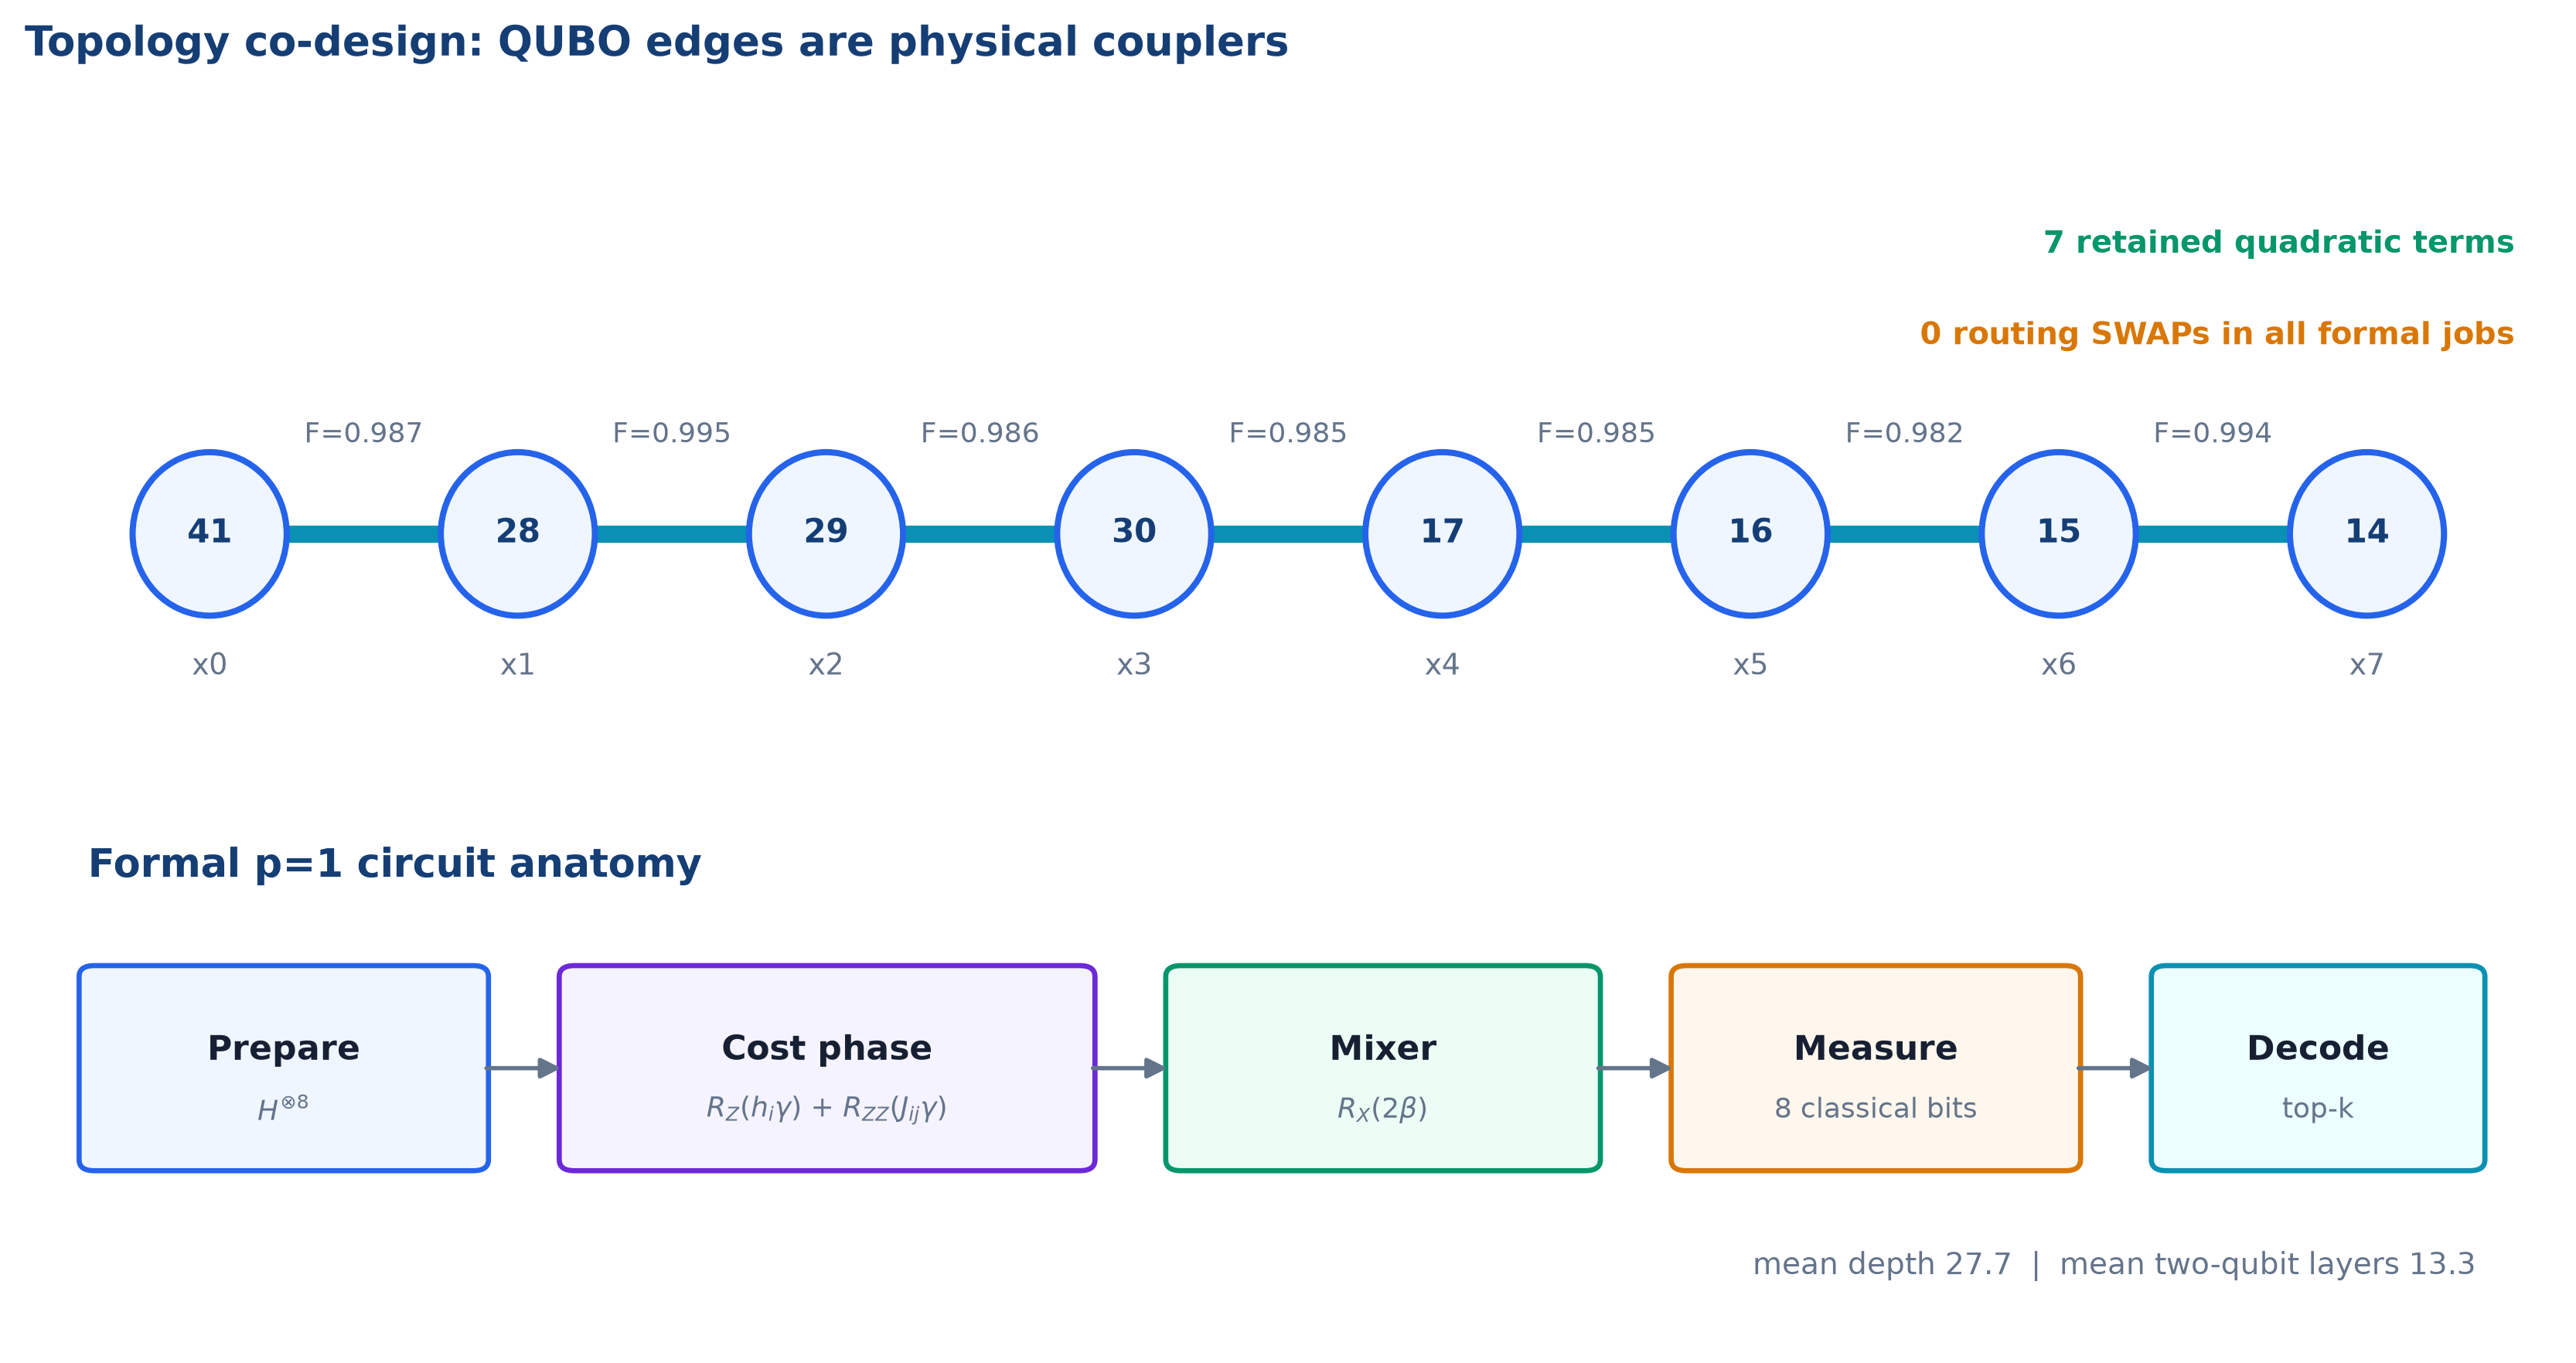
\includegraphics[width=0.94\linewidth,height=\textheight,keepaspectratio]{figures/fig03_topology_codesign.png}
\caption{逻辑变量、Baihua物理量子位链和\(p=1\)线路结构。QUBO只保留物理链直接支持的二次项。}
\end{figure}

\subsection{3.3 QAOA与参数迁移}\label{qaoaux4e0eux53c2ux6570ux8fc1ux79fb}

深度\(p\)的QAOA态为

\[
|\boldsymbol{\gamma},\boldsymbol{\beta}\rangle=
\prod_{\ell=1}^{p}e^{-i\beta_\ell H_M}e^{-i\gamma_\ell H_C}|+\rangle^{\otimes w},
\]

其中\(H_C\)由稀疏QUBO映射得到，\(H_M=\sum_i X_i\)。参数先在理想状态向量上进行确定性坐标搜索，并在相邻块之间迁移。正式配置选择\(p=1\)，原因不是``浅线路一定更优''，而是深度门控结果表明\(p=2\)尚未产生稳定增益，继续提交\(p=3\)会消耗硬件额度却没有正向趋势支撑。

\subsection{3.4 从counts到可行路线}\label{ux4ececountsux5230ux53efux884cux8defux7ebf}

每个真机任务返回4,096 shots。在线解码按频次读取前\(k=64\)个不同bitstring，对每个候选执行：

\begin{enumerate}
\def\labelenumi{\arabic{enumi}.}
\tightlist
\item
  解码为两辆车之间的局部客户分配；
\item
  若容量超限，按固定规则移动边际代价最小的客户完成修复；
\item
  重建两条受影响路线并进行相同预算的2-opt；
\item
  计算完整CVRP总距离；
\item
  仅当距离严格下降时更新当前状态。
\end{enumerate}

这一接受规则保证混合系统单调不劣。候选频率只决定评价顺序，不替代真实路线目标。

\section{4. 独立量子候选质量门槛}\label{ux72ecux7acbux91cfux5b50ux5019ux9009ux8d28ux91cfux95e8ux69db}

\subsection{4.1 门槛如何定义}\label{ux95e8ux69dbux5982ux4f55ux5b9aux4e49}

对每个宽度\(w=8\)的QUBO，完整枚举\(2^8=256\)个状态。按\((E_Q(\mathbf{x}),\mathbf{x})\)稳定排序，固定前

\[
q=\lceil 0.10\times 256\rceil=26
\]

个状态为高质量集合\(G_{0.1}\)。该集合在数学上由QUBO确定；它不读取真机counts、不读取路线改善，也不读取top-\(k\)接受结果。

真机在高质量区的概率质量为

\[
P_{\mathrm{HW}}(G_{0.1})=
\sum_{\mathbf{x}\in G_{0.1}}\frac{N_{\mathrm{HW}}(\mathbf{x})}{4096}.
\]

同一状态空间上的均匀随机基线为

\[
P_U(G_{0.1})=\frac{26}{256}=10.15625\%.
\]

因此，富集倍数\(R=P_{\mathrm{HW}}/P_U\)回答一个直接问题：从真机随机抽取一个shot，它落入预定义低能区域的概率，是没有任何量子低能偏置时的多少倍。

\subsection{4.2 统计单位与判定规则}\label{ux7edfux8ba1ux5355ux4f4dux4e0eux5224ux5b9aux89c4ux5219}

一个种子内部包含6个相关局部块，4,096个shots也来自同一线路，因此它们都不能被当成独立样本。正式统计单位是6个独立CVRP种子。我们报告种子均值、20,000次种子bootstrap区间，以及遍历\(2^6\)种符号组合的双侧精确符号翻转检验。

量子候选质量的判定规则为：硬件相对均匀随机的低能概率质量差，其95\%种子bootstrap区间下界大于0，且双侧精确\(p<0.05\)。路线改善只作为下游结果，不参与这一门槛。

需要说明的是，这一10\%门槛是在首批数据采集完成后根据评审建议引入，当前结果应视为探索性证据。门槛、统计单位和决策规则已经冻结，后续新批次可以完成真正的确认性检验。论文没有把这一时间顺序藏在脚注里，因为半决赛评审更需要可复核的证据链，而不是一个事后包装得过于完美的故事。

\section{5. 实验设计}\label{ux5b9eux9a8cux8bbeux8ba1}

\subsection{5.1 实例与正式批次}\label{ux5b9eux4f8bux4e0eux6b63ux5f0fux6279ux6b21}

实例为确定性二维欧氏CVRP，每个实例40位客户、4辆同容量车辆。种子1至10先进行局部精确余量筛查，其中种子2、3、4、7、9、10存在严格局部改善空间，被纳入正式真机集；其余4个种子没有当前DeepBlock可恢复的余量。这个筛选避免在``不存在改善答案''的局部问题上消耗真机额度，但也意味着6/6正向实例不能外推为任意CVRP实例的成功率，因此论文同时公开40\%的无余量比例。

{\def\LTcaptype{none} % do not increment counter
\begin{longtable}[]{@{}lr@{}}
\toprule\noalign{}
项目 & 正式配置 \\
\midrule\noalign{}
\endhead
\bottomrule\noalign{}
\endlastfoot
客户数 / 车辆数 & 40 / 4 \\
边界池 / 块宽 / 重叠 & 16 / 8 / 3 \\
扫描 & \(B_1\to B_2\to B_3\to B_3\to B_2\to B_1\) \\
QAOA深度 & \(p=1\) \\
每任务shots & 4,096 \\
在线候选预算 & \(k=64\) \\
正式种子 & 2, 3, 4, 7, 9, 10 \\
Baihua任务数 & 36 \\
总shots & 147,456 \\
\end{longtable}
}

\subsection{5.2 四个配对对照臂}\label{ux56dbux4e2aux914dux5bf9ux5bf9ux7167ux81c2}

{\def\LTcaptype{none} % do not increment counter
\begin{longtable}[]{@{}llrl@{}}
\toprule\noalign{}
对照臂 & 候选来源 & 状态预算 & 作用 \\
\midrule\noalign{}
\endhead
\bottomrule\noalign{}
\endlastfoot
uniform/random & 8比特均匀随机 & 4,096 & 反事实无量子偏置基线 \\
ideal & 同一QAOA的理想状态向量 & 4,096 & 估计无噪声可达分布 \\
Baihua & 超导真机counts & 4,096 & 正式量子核 \\
exact & 256状态完整枚举 & 256 & 测量局部可恢复余量 \\
\end{longtable}
}

随机、理想和Baihua臂使用相同的候选预算、容量修复、路线构造与严格接受。由于不同臂接受的移动不同，后续QUBO也不同；端到端比较以整条独立闭环为单位，不能把轨迹后半段的子问题误写成同一QUBO上的逐块配对。

\section{6. 结果：先回答量子核，再回答优化系统}\label{ux7ed3ux679cux5148ux56deux7b54ux91cfux5b50ux6838ux518dux56deux7b54ux4f18ux5316ux7cfbux7edf}

\subsection{6.1 真机低能信号}\label{ux771fux673aux4f4eux80fdux4fe1ux53f7}

\begin{figure}
\centering
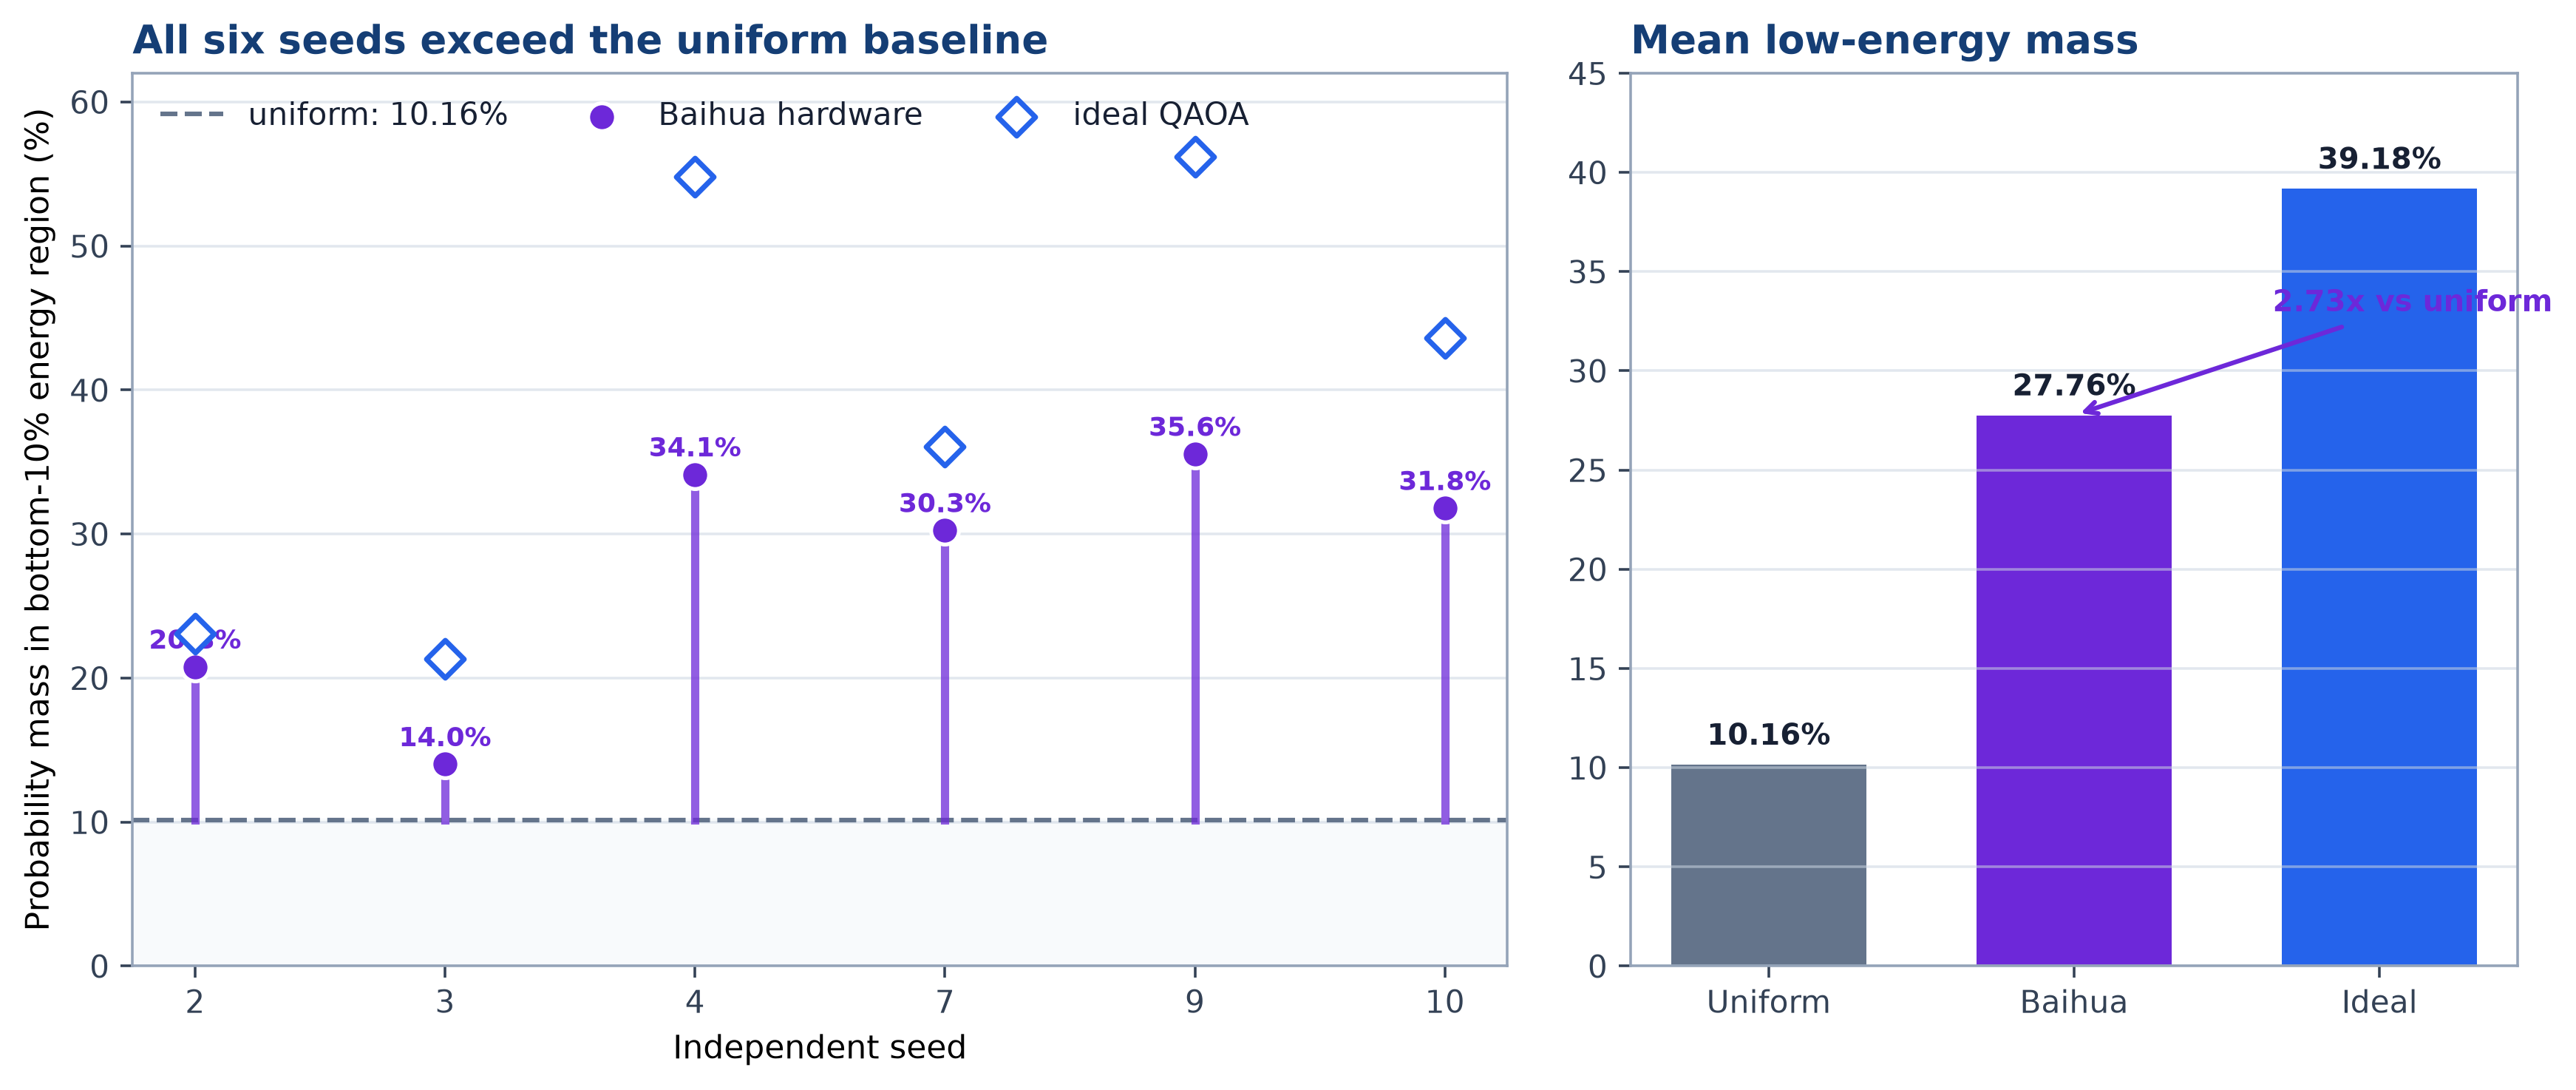
\includegraphics[width=0.96\linewidth,height=\textheight,keepaspectratio]{figures/fig04_seed_enrichment.png}
\caption{每个独立种子的最低10\%能量区域概率质量。六个种子的Baihua结果都高于10.16\%的均匀随机线。}
\end{figure}

六个种子的Baihua低能概率质量分别为20.79\%、14.02\%、34.14\%、30.26\%、35.56\%和31.80\%，全部高于10.16\%的均匀随机基线；平均值为27.76\%。理想QAOA均值为39.18\%。主结果如下：

{\def\LTcaptype{none} % do not increment counter
\begin{longtable}[]{@{}lrl@{}}
\toprule\noalign{}
指标 & 数值 & 解释 \\
\midrule\noalign{}
\endhead
\bottomrule\noalign{}
\endlastfoot
真机低能概率质量 & 27.76\% & 每个shot落入预定义高质量区的概率 \\
均匀随机概率质量 & 10.16\% & \(26/256\)，同一QUBO反事实基线 \\
真机富集倍数 & 2.73x & \(27.76/10.16\) \\
真机额外概率质量 & +17.60 pp & 比均匀随机多出的绝对概率 \\
理想QAOA概率质量 & 39.18\% & 无噪声上界参考 \\
理想超随机部分保留率 & 60.6\% & \((27.76-10.16)/(39.18-10.16)\) \\
种子方向 & 6/6为正 & 每个种子均高于随机 \\
精确符号翻转检验 & \(p=0.03125\) & \(n=6\)可达到的最小双侧\(p\)值 \\
\end{longtable}
}

这组数据给出了本项目最清晰的量子作用：若把Baihua counts替换为均匀随机，同一个低能门槛下的期望质量只有10.16\%；真实硬件将其推到27.76\%。它不是``能量降低2.73倍''，也不是``路线缩短2.73倍''，而是候选分布的低能富集。

\subsection{6.2 量子信号进入CVRP闭环}\label{ux91cfux5b50ux4fe1ux53f7ux8fdbux5165cvrpux95edux73af}

\begin{figure}
\centering
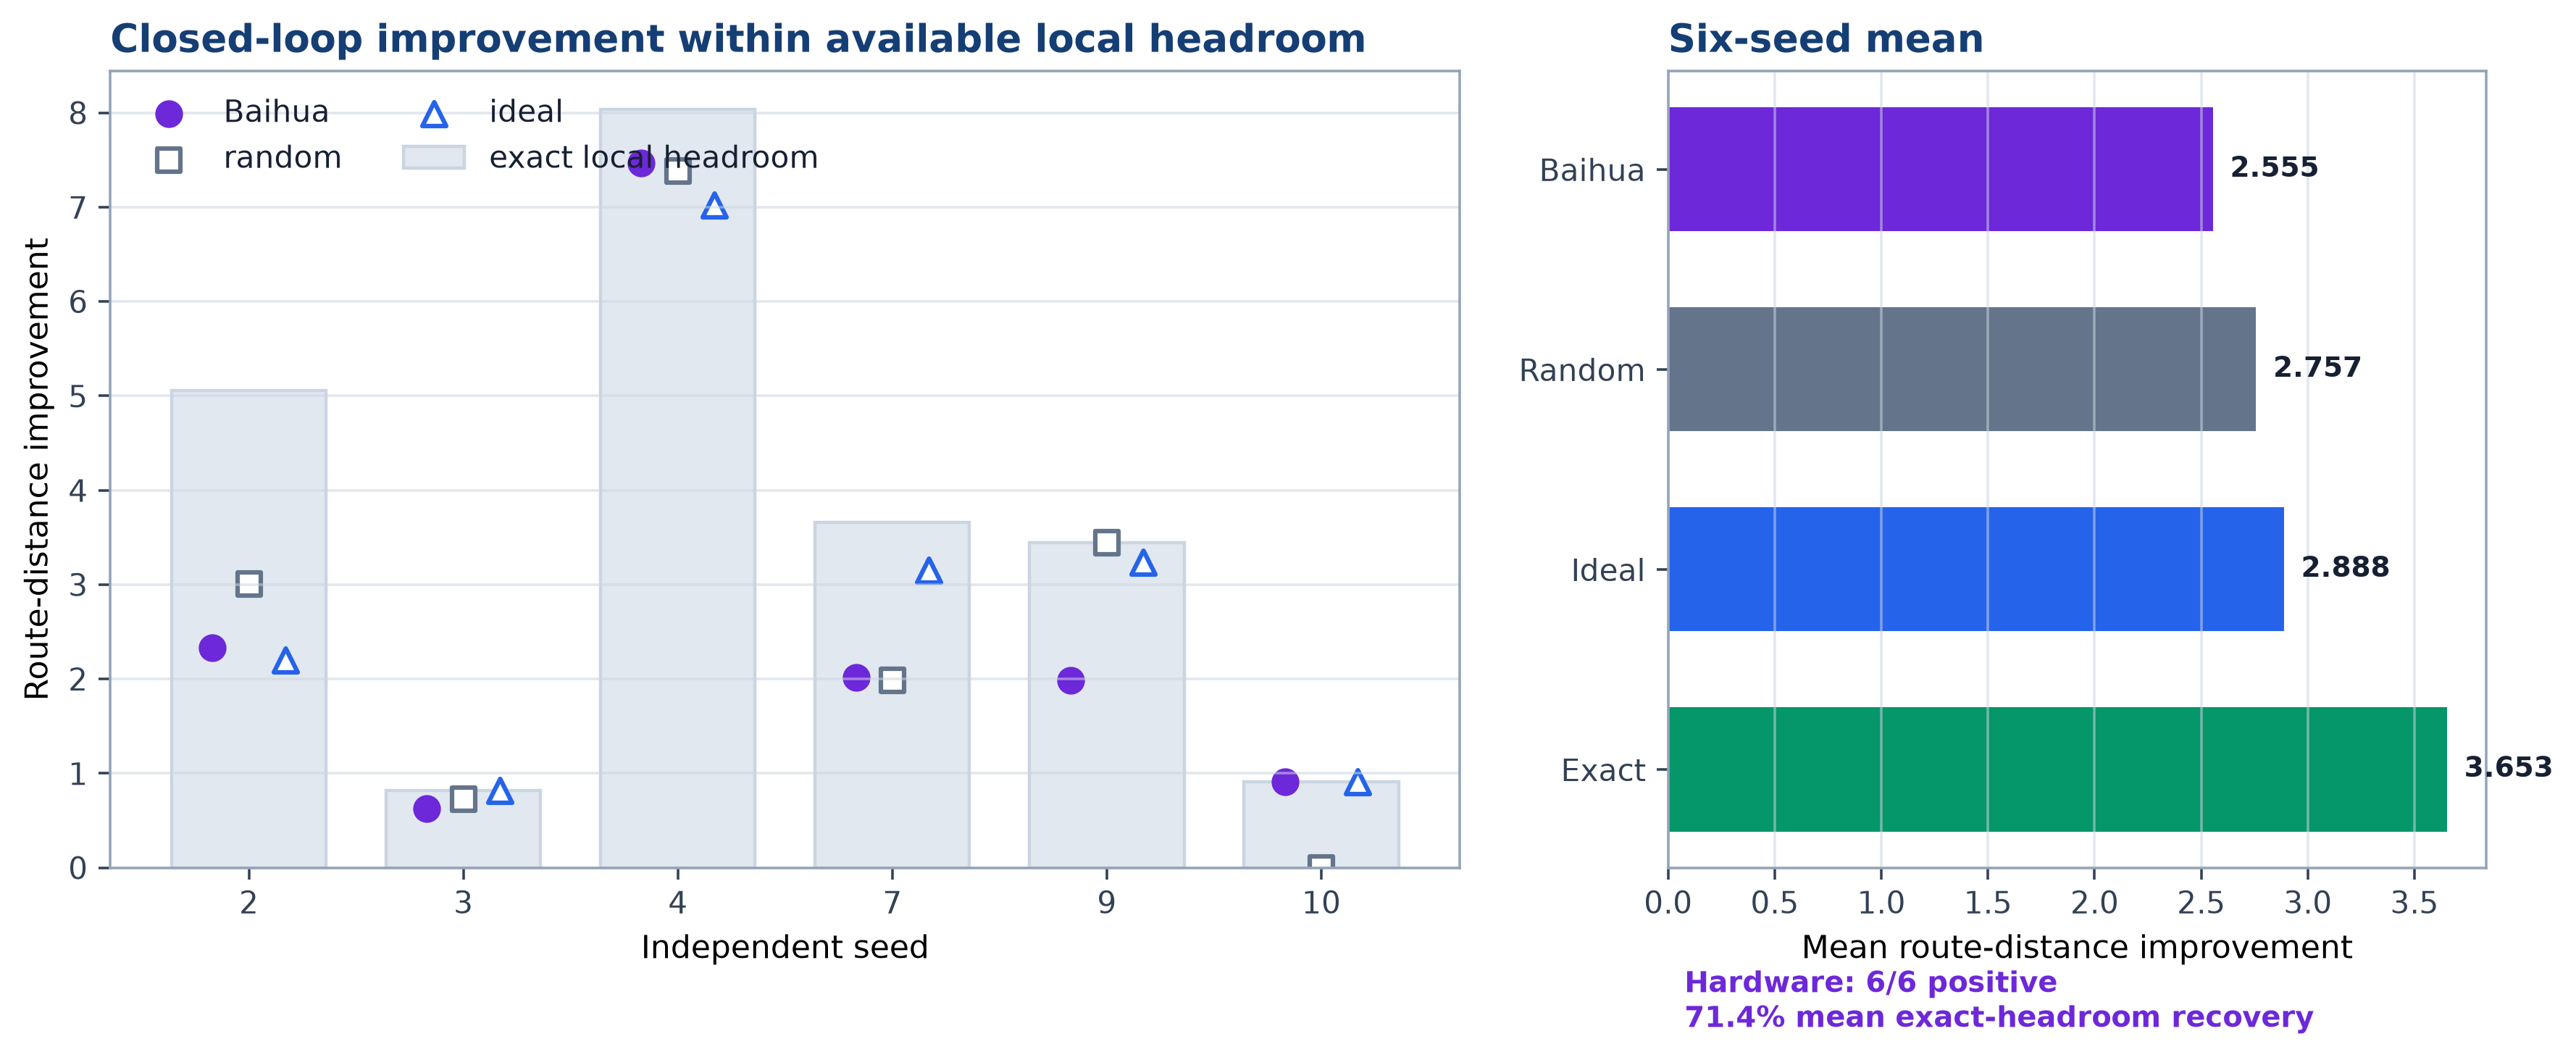
\includegraphics[width=0.96\linewidth,height=\textheight,keepaspectratio]{figures/fig05_end_to_end.png}
\caption{六个种子的可用局部精确余量，以及Baihua、随机和理想采样实际恢复的路线距离。}
\end{figure}

Baihua在6/6个正式实例上产生严格路线改善，平均距离下降2.555，平均恢复71.4\%的局部精确余量。逐种子结果表明，真机并非只在单个``幸运实例''上起作用：种子3和10达到100\%余量恢复，种子4恢复92.9\%。

端到端绝对平均改善方面，均匀随机、理想模拟和局部精确枚举分别为2.757、2.888和3.653；Baihua与随机为3胜3负，配对差异\(p=0.65625\)。这个结果不用于否定量子核，因为两项指标回答不同问题：低能门槛考察真机是否优化了它被赋予的QUBO；路线距离考察该QUBO是否准确代理了完整CVRP目标。前者显著、后者未拉开，说明瓶颈已经从``量子机有没有低能信号''转移到``代理目标能否正确排序真实路线候选''。

\subsection{6.3 候选预算比继续加深更重要}\label{ux5019ux9009ux9884ux7b97ux6bd4ux7ee7ux7eedux52a0ux6df1ux66f4ux91cdux8981}

\begin{figure}
\centering
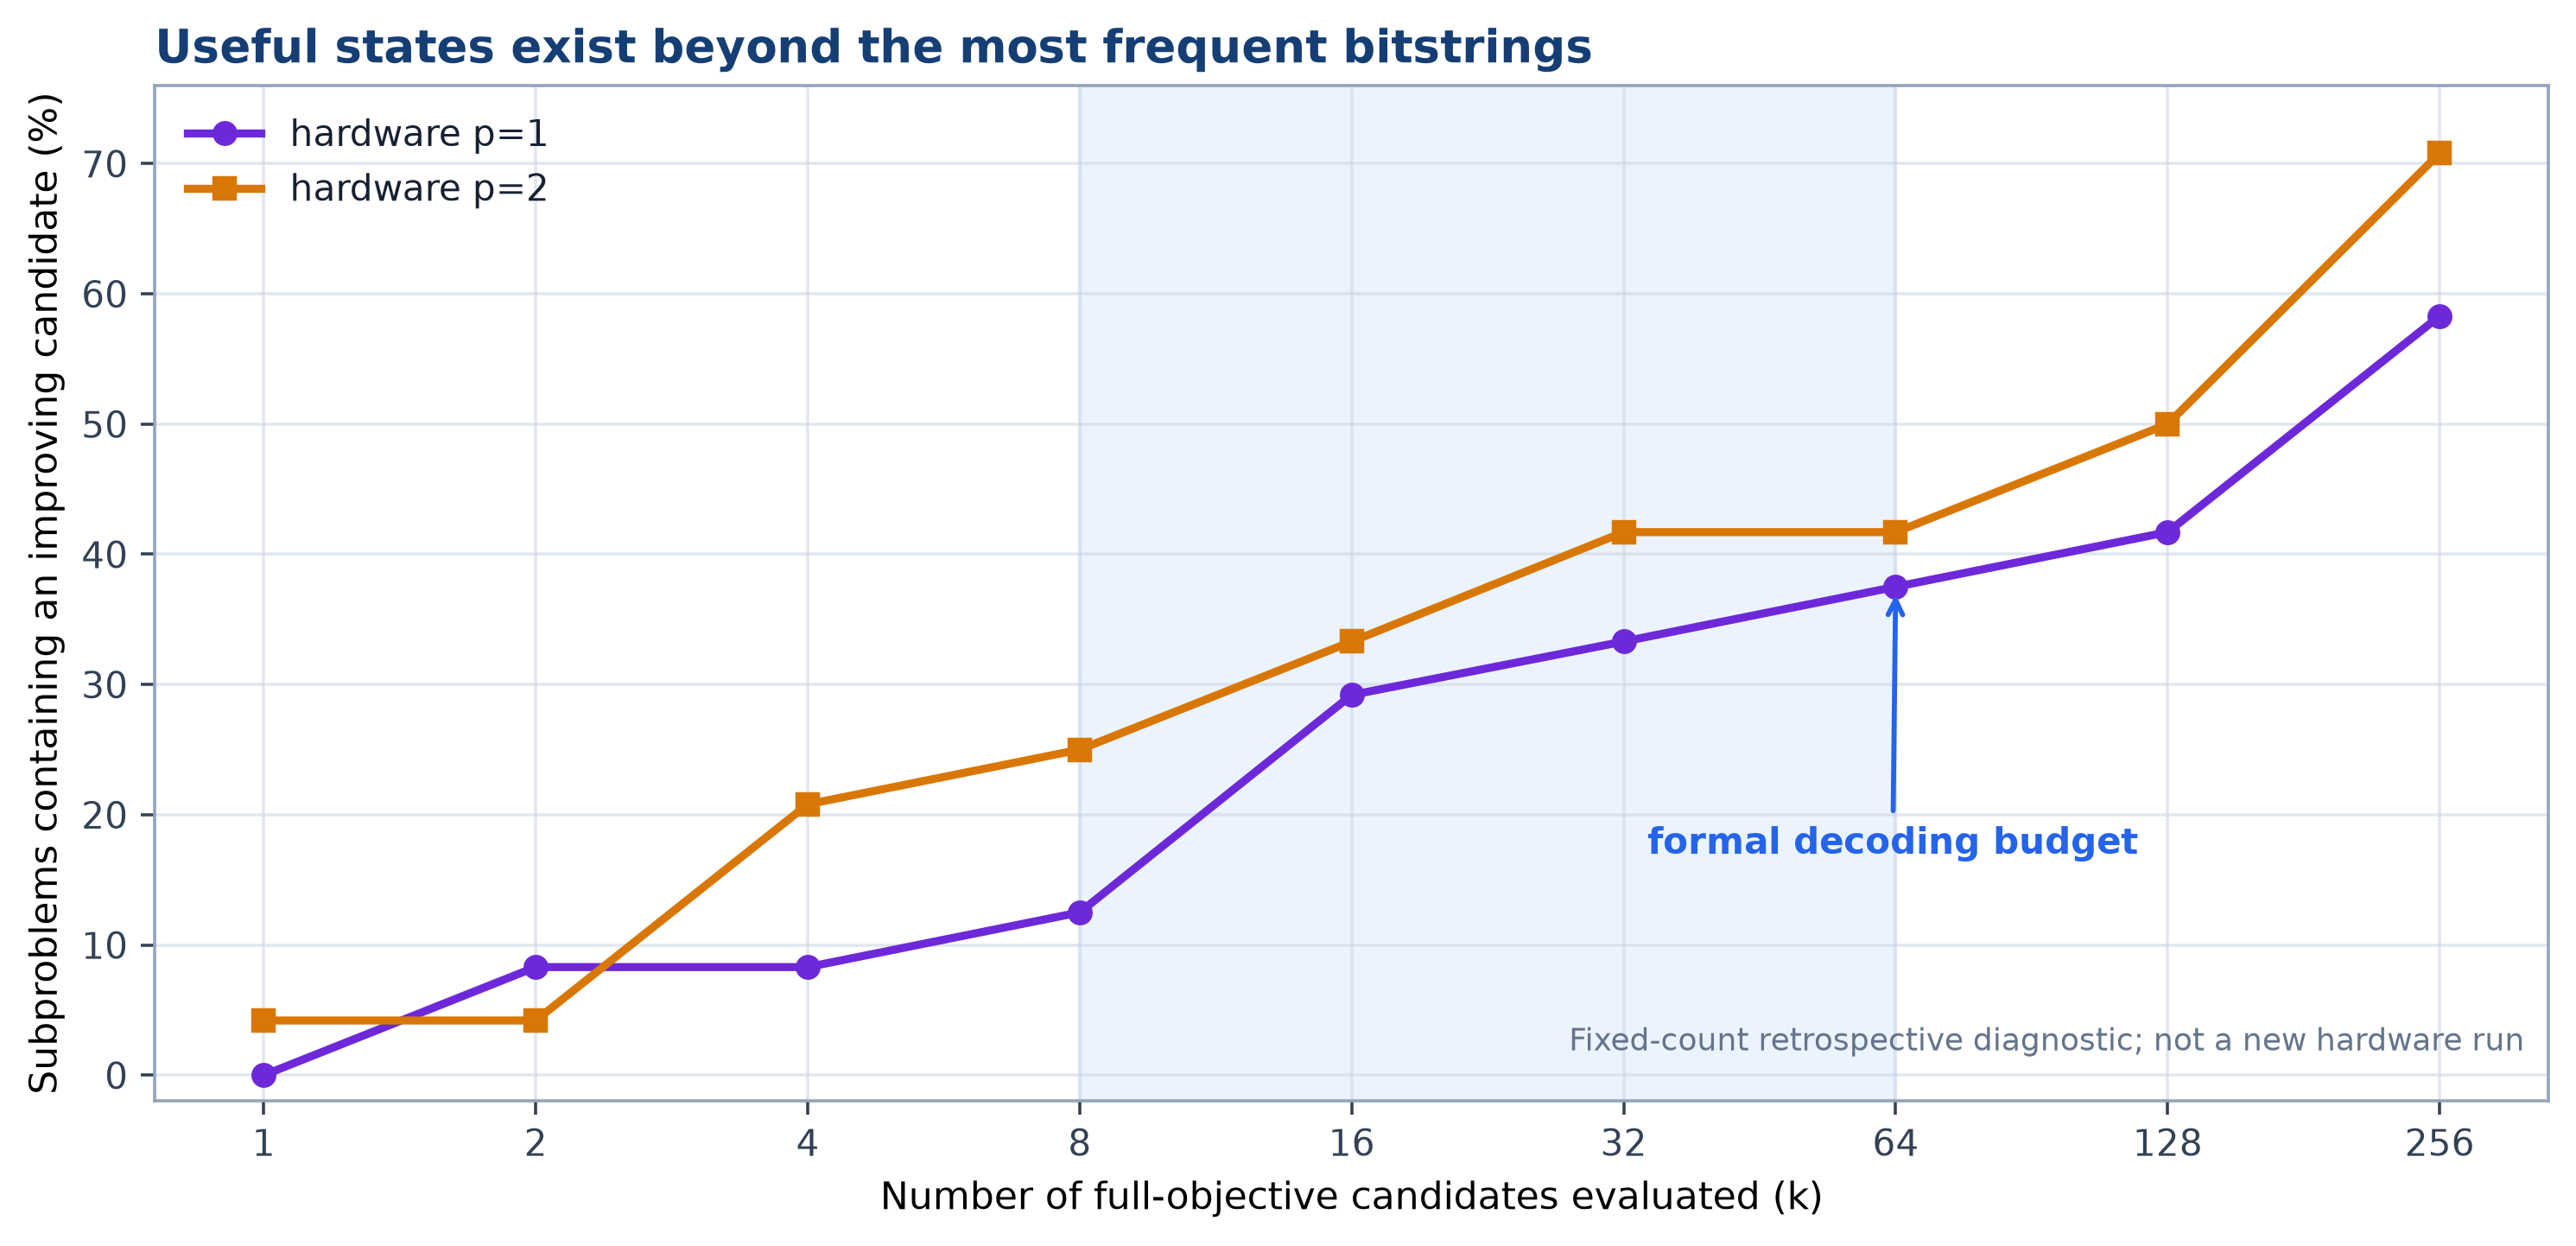
\includegraphics[width=0.9\linewidth,height=\textheight,keepaspectratio]{figures/fig06_candidate_budget.png}
\caption{固定已有counts的候选预算诊断。较低频候选中仍包含大量能改善真实路线的状态。}
\end{figure}

在\(p=1\)的24个历史硬件子问题中，只评价最高频的8个候选时，包含改善状态的子问题比例为12.5\%；\(k=16,32,64\)时分别为29.2\%、33.3\%和37.5\%；评价全部已采样状态可达到58.3\%。\(p=2\)的全量诊断达到70.8\%，却没有在\(k=8\)时形成稳定端到端收益。

种子2/3/4的闭环复算进一步给出直接干预证据：保持\(p=1\)和原始counts不变，只把在线候选预算从8提高到64，平均路线改善由1.593增至3.475，增幅118\%。同一批种子把线路从\(p=1\)加深到\(p=2\)并没有获得类似的稳定提升。对半决赛工程方案而言，这意味着有限额度应优先用于跨日确认性重复和代理校准，而不是盲目追求更深线路。

\subsection{6.4 十种子消融与失败深度}\label{ux5341ux79cdux5b50ux6d88ux878dux4e0eux5931ux8d25ux6df1ux5ea6}

\begin{figure}
\centering
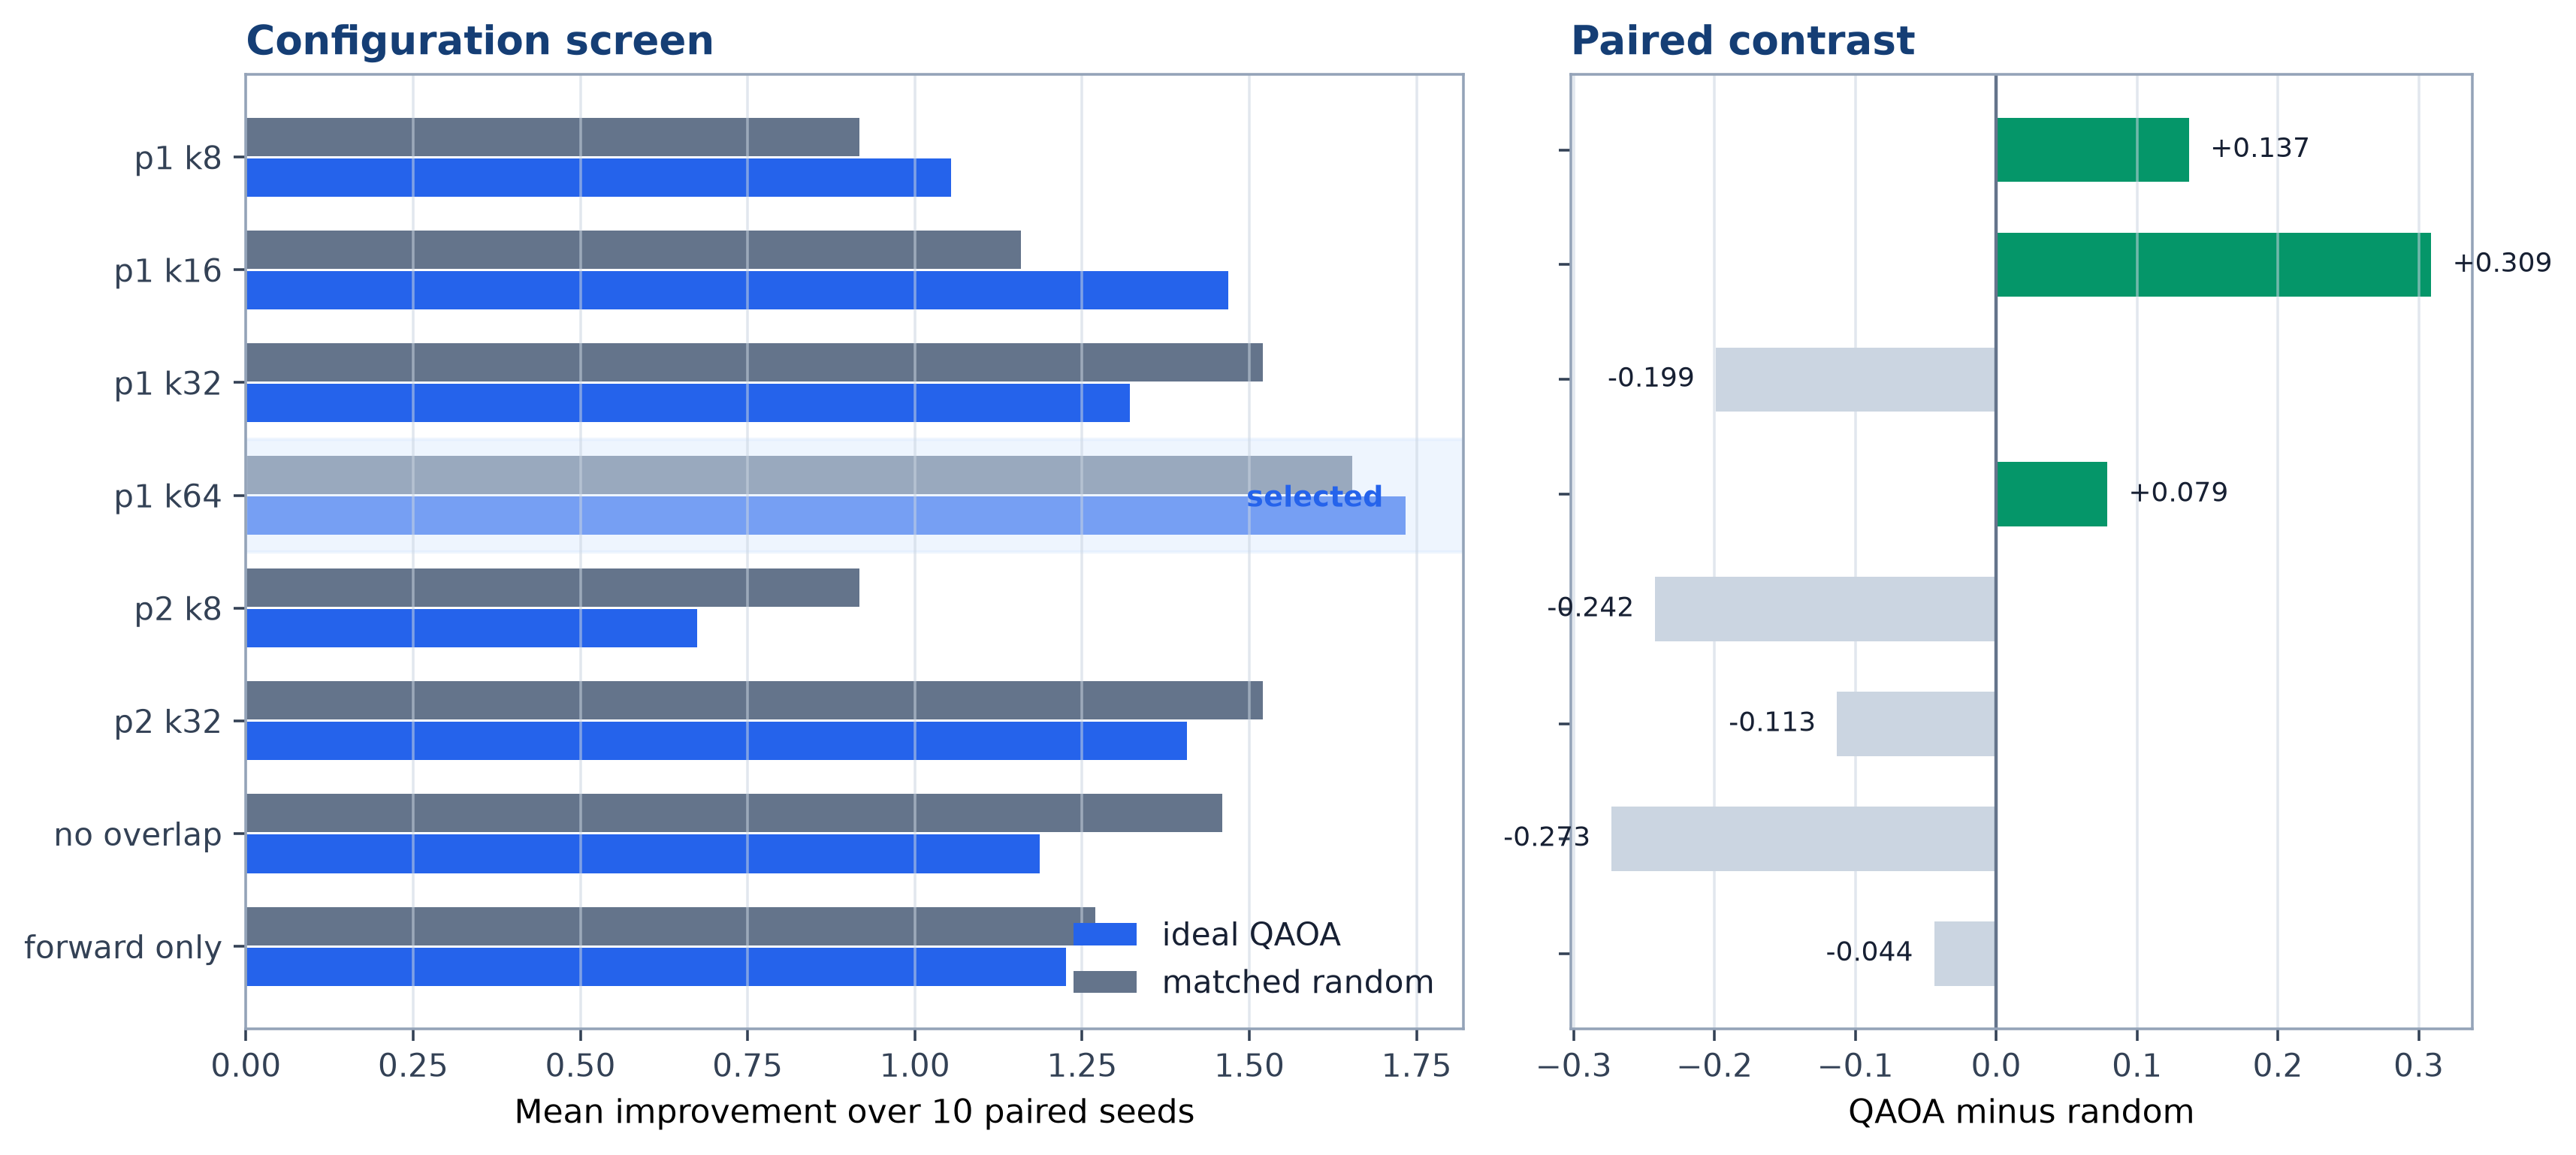
\includegraphics[width=0.92\linewidth,height=\textheight,keepaspectratio]{figures/fig07_ablation.png}
\caption{十个配对种子的配置筛选。\(p=1,k=64\)获得最高模拟平均改善；更深线路并未形成稳定优势。}
\end{figure}

\(p=1,k=16\)和\(p=1,k=64\)在十种子配对消融中超过相同预算的随机臂；\(p=1,k=32\)出现轨迹非单调，说明闭环接受会改变后续邻域，候选预算并非简单单调参数。移除3客户重叠后，模拟平均改善从1.321降至1.187；只做正向扫描时为1.226，说明重叠和双向扫描提供了结构价值。

\(p=2\)在种子3上恢复约89.3\%的精确余量并超过随机与理想模拟，但种子2和4退化。按照预先使用的``\(p=2\)未稳定优于\(p=1\)''门控，项目没有继续提交\(p=3\)任务。这个停止决定保留在论文中，因为它展示了算法选择由数据门控，而不是由``深线路看起来更量子''驱动。

\section{7. 为什么这项工作适合``量子+优化''赛道}\label{ux4e3aux4ec0ux4e48ux8fd9ux9879ux5de5ux4f5cux9002ux5408ux91cfux5b50ux4f18ux5316ux8d5bux9053}

\subsection{7.1 量子不是装饰性调用}\label{ux91cfux5b50ux4e0dux662fux88c5ux9970ux6027ux8c03ux7528}

如果量子模块只是把随机bitstring交给经典修复，低能区域的概率质量应接近10.16\%。正式结果为27.76\%，并且6个种子全部为正。这个差异在不执行容量修复、不构造路线、不读取接受结果时已经存在，所以不能由经典后处理制造。

进一步地，量子counts处在逐块状态转移的因果链上：被接受的bitstring改变客户归属，更新后的路线又决定下一个边界块和QUBO。删除量子模块并用均匀随机替代，会同时改变候选分布和后续轨迹。这是一个真正的混合优化系统，而不是在经典答案生成后附加一段量子线路。

\subsection{7.2 物理拓扑进入了优化模型}\label{ux7269ux7406ux62d3ux6251ux8fdbux5165ux4e86ux4f18ux5316ux6a21ux578b}

许多QAOA项目把映射当作编译器的末端工作。DeepBlock把拓扑提前到QUBO构造：硬件链决定允许的二次项，校准保真度决定物理子图，0 SWAP不是一次幸运编译，而是模型结构的直接结果。这种``问题-线路-硬件''共设计是本项目最容易迁移到更大设备的部分：未来可将单链替换为树、格或多个链块，而不改变经典主框架。

\subsection{7.3 证据比单张最优路线更完整}\label{ux8bc1ux636eux6bd4ux5355ux5f20ux6700ux4f18ux8defux7ebfux66f4ux5b8cux6574}

\begin{figure}
\centering
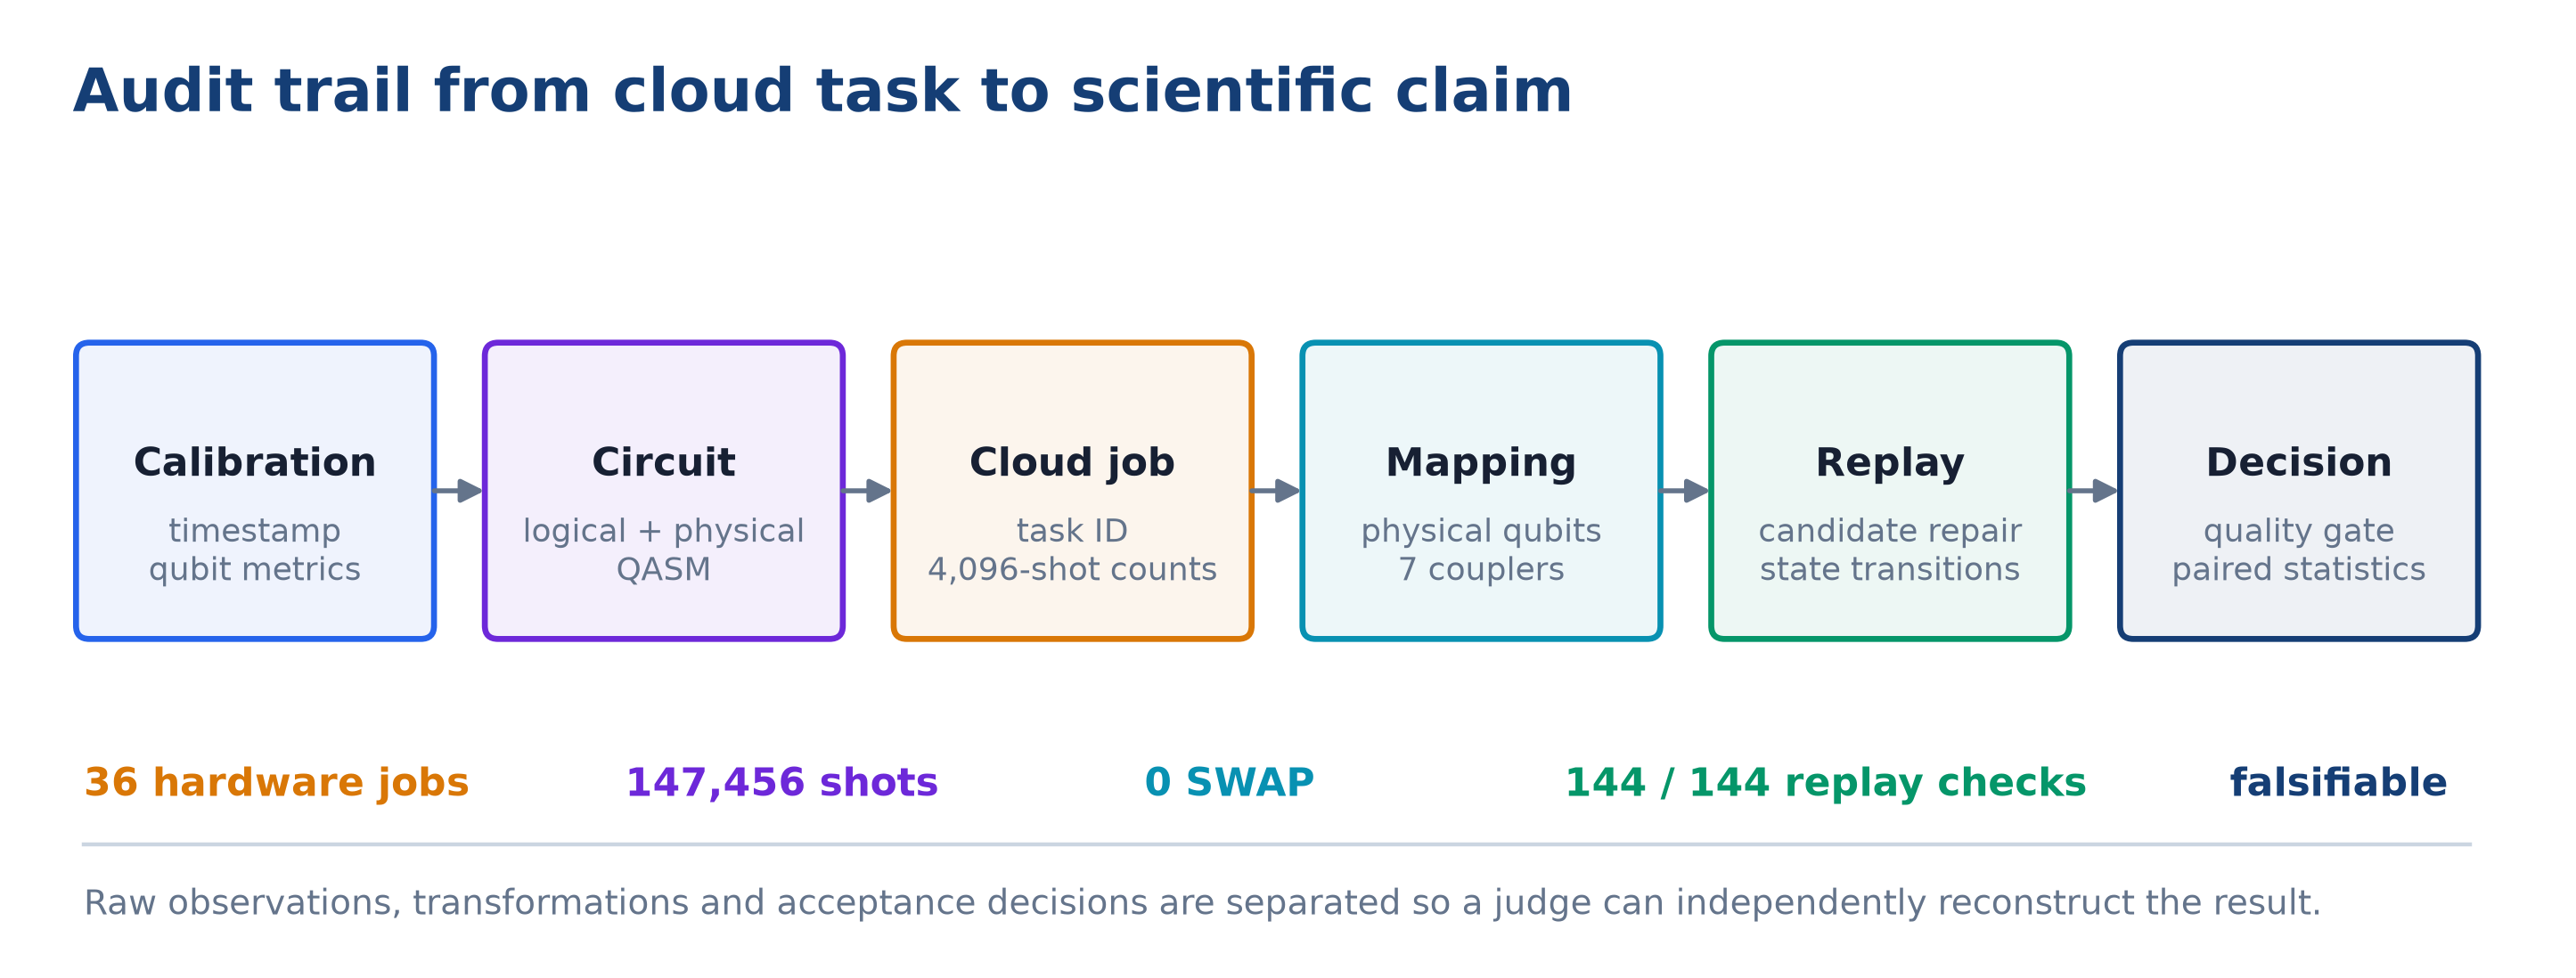
\includegraphics[width=0.94\linewidth,height=\textheight,keepaspectratio]{figures/fig08_reproducibility_chain.png}
\caption{从校准、线路、云端任务到统计判定的证据链。所有关键变换都可由归档工件离线重建。}
\end{figure}

每个真机子问题保存以下工件：校准时间和量子位指标、逻辑QASM、物理QASM、物理量子位与耦合映射、任务ID、原始counts、QAOA参数、代理QUBO、候选容量修复、真实距离评价、接受前后客户分配。四个实验臂共形成144条重放记录，144/144通过bitstring解释、best-of-shots和状态转移一致性检查。

这条证据链能让评委区分三件经常混在一起的事：线路是否提交成功、counts是否真的来自硬件、counts是否改变了优化状态。可复现性在这里不是附录装饰，而是量子贡献能够被相信的前提。

\section{8. 当前短板与半决赛后的决定性实验}\label{ux5f53ux524dux77edux677fux4e0eux534aux51b3ux8d5bux540eux7684ux51b3ux5b9aux6027ux5b9eux9a8c}

\subsection{8.1 真正的短板是代理目标错位}\label{ux771fux6b63ux7684ux77edux677fux662fux4ee3ux7406ux76eeux6807ux9519ux4f4d}

历史硬件子问题中，QUBO能量与真实路线距离的Spearman相关系数接近0（\(p=1\)约为\(-0.025\)，\(p=2\)约为\(-0.038\)）。这解释了为什么量子机明显富集QUBO低能态，却尚未在端到端路线指标上拉开随机基线。量子机正在完成它收到的任务，问题在于代理任务还没有稳定表达真实CVRP增量。

下一阶段不应继续堆罚项，而应使用真实路线增量监督代理系数。具体方案是：在训练种子上枚举8比特局部状态，得到\(\Delta L(\mathbf{x})\)；以排序损失或岭回归拟合\(h_i,J_{ij}\)，同时加入物理边稀疏约束；冻结代理后在独立种子上检验能量与\(\Delta L\)的秩相关，并比较相同完整目标评价预算下的sample efficiency。只有代理相关性先过门槛，量子低能富集才有机会稳定转化为路线优势。

\subsection{8.2 需要确认性而非重复利用旧数据}\label{ux9700ux8981ux786eux8ba4ux6027ux800cux975eux91cdux590dux5229ux7528ux65e7ux6570ux636e}

最低10\%能量门槛已经冻结。半决赛后最有价值的新真机批次应满足：不少于30个预注册种子，包含有余量和无余量实例；跨3至5个校准日期；同一QUBO分别执行Baihua、均匀随机和理想模拟；主统计仍以种子为单位；不在看到counts后修改10\%阈值。若硬件减随机的95\%bootstrap下界仍大于0且精确\(p<0.05\)，探索性结果即可升级为确认性证据。

\subsection{8.3 规模扩展不能靠8比特枚举}\label{ux89c4ux6a21ux6269ux5c55ux4e0dux80fdux97608ux6bd4ux7279ux679aux4e3e}

当前每个量子核只有8个真实决策位，256个状态可被经典枚举，因此不能声称计算复杂度优势。扩展路线是把DeepBlock从单链8位升级到14至20位的树状或多链物理子图，并用分支限界、禁忌搜索和重要性随机作为同预算基线。届时评测重点应从``是否找到最优''转为固定时间或固定完整目标调用次数下的最优差距、成功率和尾部风险。

\section{9. 结论}\label{ux7ed3ux8bba}

DeepBlock给出的不是一条被量子术语包装的经典路线，而是一套能够指出量子处理器具体贡献位置的混合优化实验。Baihua在36个正式任务中完成147,456 shots，全部0 SWAP；在不借助路线接受结果的独立门槛下，真机将最低10\% QUBO能量区域的概率质量从均匀随机的10.16\%提高到27.76\%，形成2.73倍富集，6/6个种子方向一致。该分布信号进入容量修复、真实路线评价和单调接受组成的闭环，在6/6个有余量实例上产生路线改善，并恢复71.4\%的局部精确余量。

这项工作当前最重要的科学判断也很明确：硬件已经产生可测的优化偏置，端到端上限却由代理QUBO与真实CVRP距离的错位决定。比继续加深线路更有效的动作，是学习一个能排序真实路线增量的拓扑稀疏代理，并用冻结阈值开展跨日确认性真机实验。对于``量子+优化''赛道，这种把正结果、失败边界和下一步决定性实验放在同一证据链中的方案，比单独展示一次最优采样更接近可迁移、可审计的量子优化工程。

\section{参考文献}\label{ux53c2ux8003ux6587ux732e}

\begin{enumerate}
\def\labelenumi{\arabic{enumi}.}
\tightlist
\item
  Dantzig G B, Ramser J H. The Truck Dispatching Problem. \emph{Management Science}, 1959, 6(1): 80-91. DOI: 10.1287/mnsc.6.1.80.
\item
  Laporte G. Fifty Years of Vehicle Routing. \emph{Transportation Science}, 2009, 43(4): 408-416. DOI: 10.1287/trsc.1090.0301.
\item
  Preskill J. Quantum Computing in the NISQ Era and Beyond. \emph{Quantum}, 2018, 2: 79. DOI: 10.22331/q-2018-08-06-79.
\item
  Glover F, Kochenberger G, Du Y. Quantum Bridge Analytics I: A Tutorial on Formulating and Using QUBO Models. \emph{4OR}, 2019, 17: 335-371. DOI: 10.1007/s10288-019-00424-y.
\item
  Lucas A. Ising Formulations of Many NP Problems. \emph{Frontiers in Physics}, 2014, 2: 5. DOI: 10.3389/fphy.2014.00005.
\item
  Farhi E, Goldstone J, Gutmann S. A Quantum Approximate Optimization Algorithm. arXiv:1411.4028, 2014.
\item
  Hadfield S, Wang Z, O'Gorman B, et al.~From the Quantum Approximate Optimization Algorithm to a Quantum Alternating Operator Ansatz. \emph{Algorithms}, 2019, 12(2): 34. DOI: 10.3390/a12020034.
\item
  Zhou L, Wang S T, Choi S, et al.~Quantum Approximate Optimization Algorithm: Performance, Mechanism, and Implementation on Near-Term Devices. \emph{Physical Review X}, 2020, 10: 021067.
\item
  Cerezo M, Arrasmith A, Babbush R, et al.~Variational Quantum Algorithms. \emph{Nature Reviews Physics}, 2021, 3: 625-644.
\item
  Xu H Z, Zhuang W F, Wang Z A, et al.~Quafu-Qcover: Explore Combinatorial Optimization Problems on Cloud-Based Quantum Computers. \emph{Chinese Physics B}, 2024, 33(5): 050302.
\item
  Feld S, Roch C, Gabor T, et al.~A Hybrid Solution Method for the Capacitated Vehicle Routing Problem Using a Quantum Annealer. \emph{Frontiers in ICT}, 2019, 6: 13.
\item
  Harwood S, Gambella C, Trenev D, et al.~Formulating and Solving Routing Problems on Quantum Computers. \emph{IEEE Transactions on Quantum Engineering}, 2021, 2: 3100118.
\item
  Azad U, Behera B K, Ahmed E A, et al.~Solving Vehicle Routing Problem Using Quantum Approximate Optimization Algorithm. \emph{IEEE Transactions on Intelligent Transportation Systems}, 2023, 24: 7564-7573.
\item
  Fitzek D, Ghandriz T, Laine L, et al.~Applying Quantum Approximate Optimization to the Heterogeneous Vehicle Routing Problem. \emph{Scientific Reports}, 2024, 14: 25415.
\item
  Xie N, Lee X, Cai D, et al.~A Feasibility-Preserved Quantum Approximate Solver for the Capacitated Vehicle Routing Problem. arXiv:2308.08785, 2023.
\item
  Huang W H, Matsuyama H, Yamashiro Y. Solving Capacitated Vehicle Routing Problem with Quantum Alternating Operator Ansatz and Column Generation. arXiv:2503.17051, 2025.
\end{enumerate}

\section{附录A：结果与复现目录}\label{ux9644ux5f55aux7ed3ux679cux4e0eux590dux73b0ux76eeux5f55}

\begin{itemize}
\tightlist
\item
  正式真机批次：\texttt{results/baihua\_hardware\_p1\_k64\_seeds2\_3\_4\_20260801}；
\item
  正式真机批次：\texttt{results/baihua\_hardware\_p1\_k64\_seeds7\_9\_10\_20260801}；
\item
  候选质量证据：\texttt{results/baihua\_quantum\_candidate\_quality\_20260801}；
\item
  半决赛汇总包：\texttt{results/baihua\_competition\_package\_20260801}；
\item
  六种子四臂结果：\texttt{formal\_seed\_results.csv}；
\item
  冻结确认协议：\texttt{frozen\_confirmatory\_protocol.json}；
\item
  论文图表均由归档CSV/JSON重建，不会提交新的云端任务。
\end{itemize}

\section{附录B：冻结确认性判定}\label{ux9644ux5f55bux51bbux7ed3ux786eux8ba4ux6027ux5224ux5b9a}

\begin{enumerate}
\def\labelenumi{\arabic{enumi}.}
\tightlist
\item
  高质量集合固定为每个QUBO最低10\%能量秩，不改为5\%、20\%或事后最优分位数；
\item
  主统计单位为独立CVRP种子，不把子问题或shots当作独立样本；
\item
  主比较为同一QUBO完整状态空间上的均匀随机分布；
\item
  判定规则为硬件减随机的95\%种子bootstrap下界大于0，且双侧精确符号翻转检验\(p<0.05\)；
\item
  路线改善、容量修复和组合门槛只作为下游诊断，不改变量子候选质量判定；
\item
  所有预注册种子进入主结果；无局部余量实例按零改善纳入总体端到端统计。
\end{enumerate}

\end{document}
